% Options for packages loaded elsewhere
% Options for packages loaded elsewhere
\PassOptionsToPackage{unicode}{hyperref}
\PassOptionsToPackage{hyphens}{url}
\PassOptionsToPackage{dvipsnames,svgnames,x11names}{xcolor}
%
\documentclass[
  11pt,
  a4paper,
]{article}
\usepackage{xcolor}
\usepackage[margin=25mm]{geometry}
\usepackage{amsmath,amssymb}
\setcounter{secnumdepth}{3}
\usepackage{iftex}
\ifPDFTeX
  \usepackage[T1]{fontenc}
  \usepackage[utf8]{inputenc}
  \usepackage{textcomp} % provide euro and other symbols
\else % if luatex or xetex
  \usepackage{unicode-math} % this also loads fontspec
  \defaultfontfeatures{Scale=MatchLowercase}
  \defaultfontfeatures[\rmfamily]{Ligatures=TeX,Scale=1}
\fi
\usepackage{lmodern}
\ifPDFTeX\else
  % xetex/luatex font selection
\fi
% Use upquote if available, for straight quotes in verbatim environments
\IfFileExists{upquote.sty}{\usepackage{upquote}}{}
\IfFileExists{microtype.sty}{% use microtype if available
  \usepackage[]{microtype}
  \UseMicrotypeSet[protrusion]{basicmath} % disable protrusion for tt fonts
}{}
\makeatletter
\@ifundefined{KOMAClassName}{% if non-KOMA class
  \IfFileExists{parskip.sty}{%
    \usepackage{parskip}
  }{% else
    \setlength{\parindent}{0pt}
    \setlength{\parskip}{6pt plus 2pt minus 1pt}}
}{% if KOMA class
  \KOMAoptions{parskip=half}}
\makeatother
% Make \paragraph and \subparagraph free-standing
\makeatletter
\ifx\paragraph\undefined\else
  \let\oldparagraph\paragraph
  \renewcommand{\paragraph}{
    \@ifstar
      \xxxParagraphStar
      \xxxParagraphNoStar
  }
  \newcommand{\xxxParagraphStar}[1]{\oldparagraph*{#1}\mbox{}}
  \newcommand{\xxxParagraphNoStar}[1]{\oldparagraph{#1}\mbox{}}
\fi
\ifx\subparagraph\undefined\else
  \let\oldsubparagraph\subparagraph
  \renewcommand{\subparagraph}{
    \@ifstar
      \xxxSubParagraphStar
      \xxxSubParagraphNoStar
  }
  \newcommand{\xxxSubParagraphStar}[1]{\oldsubparagraph*{#1}\mbox{}}
  \newcommand{\xxxSubParagraphNoStar}[1]{\oldsubparagraph{#1}\mbox{}}
\fi
\makeatother


\usepackage{longtable,booktabs,array}
\newcounter{none} % for unnumbered tables
\usepackage{calc} % for calculating minipage widths
% Correct order of tables after \paragraph or \subparagraph
\usepackage{etoolbox}
\makeatletter
\patchcmd\longtable{\par}{\if@noskipsec\mbox{}\fi\par}{}{}
\makeatother
% Allow footnotes in longtable head/foot
\IfFileExists{footnotehyper.sty}{\usepackage{footnotehyper}}{\usepackage{footnote}}
\makesavenoteenv{longtable}
\usepackage{graphicx}
\makeatletter
\newsavebox\pandoc@box
\newcommand*\pandocbounded[1]{% scales image to fit in text height/width
  \sbox\pandoc@box{#1}%
  \Gscale@div\@tempa{\textheight}{\dimexpr\ht\pandoc@box+\dp\pandoc@box\relax}%
  \Gscale@div\@tempb{\linewidth}{\wd\pandoc@box}%
  \ifdim\@tempb\p@<\@tempa\p@\let\@tempa\@tempb\fi% select the smaller of both
  \ifdim\@tempa\p@<\p@\scalebox{\@tempa}{\usebox\pandoc@box}%
  \else\usebox{\pandoc@box}%
  \fi%
}
% Set default figure placement to htbp
\def\fps@figure{htbp}
\makeatother


% definitions for citeproc citations
\NewDocumentCommand\citeproctext{}{}
\NewDocumentCommand\citeproc{mm}{%
  \begingroup\def\citeproctext{#2}\cite{#1}\endgroup}
\makeatletter
 % allow citations to break across lines
 \let\@cite@ofmt\@firstofone
 % avoid brackets around text for \cite:
 \def\@biblabel#1{}
 \def\@cite#1#2{{#1\if@tempswa , #2\fi}}
\makeatother
\newlength{\cslhangindent}
\setlength{\cslhangindent}{1.5em}
\newlength{\csllabelwidth}
\setlength{\csllabelwidth}{3em}
\newenvironment{CSLReferences}[2] % #1 hanging-indent, #2 entry-spacing
 {\begin{list}{}{%
  \setlength{\itemindent}{0pt}
  \setlength{\leftmargin}{0pt}
  \setlength{\parsep}{0pt}
  % turn on hanging indent if param 1 is 1
  \ifodd #1
   \setlength{\leftmargin}{\cslhangindent}
   \setlength{\itemindent}{-1\cslhangindent}
  \fi
  % set entry spacing
  \setlength{\itemsep}{#2\baselineskip}}}
 {\end{list}}
\usepackage{calc}
\newcommand{\CSLBlock}[1]{\hfill\break\parbox[t]{\linewidth}{\strut\ignorespaces#1\strut}}
\newcommand{\CSLLeftMargin}[1]{\parbox[t]{\csllabelwidth}{\strut#1\strut}}
\newcommand{\CSLRightInline}[1]{\parbox[t]{\linewidth - \csllabelwidth}{\strut#1\strut}}
\newcommand{\CSLIndent}[1]{\hspace{\cslhangindent}#1}



\setlength{\emergencystretch}{3em} % prevent overfull lines

\providecommand{\tightlist}{%
  \setlength{\itemsep}{0pt}\setlength{\parskip}{0pt}}



 


\usepackage{booktabs}
\usepackage{longtable}
\usepackage{array}
\usepackage{multirow}
\usepackage{wrapfig}
\usepackage{float}
\usepackage{colortbl}
\usepackage{pdflscape}
\usepackage{tabu}
\usepackage{threeparttable}
\usepackage{threeparttablex}
\usepackage[normalem]{ulem}
\usepackage{makecell}
\usepackage{xcolor}
\renewcommand{\baselinestretch}{1.1}
\usepackage{microtype}
\frenchspacing
\usepackage{graphicx}
\usepackage{xcolor}
\usepackage{amsmath,amssymb}
\usepackage{booktabs}
\usepackage{longtable}
\usepackage{array}
\usepackage{multirow}
\usepackage{makecell}
\usepackage{pdflscape}
\usepackage{float}
\usepackage{fancyhdr}
\makeatletter
\@ifpackageloaded{caption}{}{\usepackage{caption}}
\AtBeginDocument{%
\ifdefined\contentsname
  \renewcommand*\contentsname{Table of contents}
\else
  \newcommand\contentsname{Table of contents}
\fi
\ifdefined\listfigurename
  \renewcommand*\listfigurename{List of Figures}
\else
  \newcommand\listfigurename{List of Figures}
\fi
\ifdefined\listtablename
  \renewcommand*\listtablename{List of Tables}
\else
  \newcommand\listtablename{List of Tables}
\fi
\ifdefined\figurename
  \renewcommand*\figurename{Figure}
\else
  \newcommand\figurename{Figure}
\fi
\ifdefined\tablename
  \renewcommand*\tablename{Table}
\else
  \newcommand\tablename{Table}
\fi
}
\@ifpackageloaded{float}{}{\usepackage{float}}
\floatstyle{ruled}
\@ifundefined{c@chapter}{\newfloat{codelisting}{h}{lop}}{\newfloat{codelisting}{h}{lop}[chapter]}
\floatname{codelisting}{Listing}
\newcommand*\listoflistings{\listof{codelisting}{List of Listings}}
\makeatother
\makeatletter
\makeatother
\makeatletter
\@ifpackageloaded{caption}{}{\usepackage{caption}}
\@ifpackageloaded{subcaption}{}{\usepackage{subcaption}}
\makeatother
\usepackage{bookmark}
\IfFileExists{xurl.sty}{\usepackage{xurl}}{} % add URL line breaks if available
\urlstyle{same}
\hypersetup{
  colorlinks=true,
  linkcolor={blue},
  filecolor={Maroon},
  citecolor={Blue},
  urlcolor={Blue},
  pdfcreator={LaTeX via pandoc}}


\author{}
\date{}
\begin{document}


\section{Abstract}\label{abstract}

Under-five mortality has fallen globally, but large inequalities remain
between and within countries. Standard decomposition methods can show
which variables contribute to socioeconomic inequality, but they are
less direct in showing how determinants combine into subgroups. This
thesis developed and applied a tree-based method for analysing
socioeconomic inequality in under-five mortality. The method used the
concentration index as the impurity measure in recursive partitioning,
so that splits were chosen to reduce within-node socioeconomic
inequality in the outcome. The method was applied to child-level data
from the Democratic Republic of the Congo DHS phase V survey, using
under-five mortality as the outcome and the DHS wealth index as the
socioeconomic ranking variable.

The analysis compared indirect decomposition methods with direct
concentration-index trees and forests. In the indirect methods, a model
was fitted first, either a generalised linear model or a predictive
model such as a random forest, and the fitted model was then used to
decompose inequality. The regression decomposition placed the greatest
weight on the mother's education and the father's agricultural
occupation. The SHAP decomposition was less concentrated on these two
variables. Residence, household wealth, mother's education, skilled
birth attendance, and parental occupation all appeared across the
criteria.

The direct trees added the subgroup part of the analysis. The
rank-dependent trees based on standard concentration index(\(CI\)),
generalised concentration index(\(CIg\)), and corrected concentration
index(\(CIc\)) split mainly through mother's education, father's
agricultural occupation, skilled birth attendance, household wealth, and
Katanga. The high-mortality branch was made up of children whose mothers
had no education, who lived in low-wealth households, and who resided in
Katanga. This pattern was clear in the fitted data, but it did not carry
well to the validation folds. The level-dependent concentration
index(\(L\)) method gave a different tree. It was first split by
residence, then by occupation, wealth, and province. The \(L\) tree and
forest both kept positive validation gains, so the level-dependent
result was treated as the more stable direct result in this application.

The thesis shows that concentration-index trees can be used to add
subgroup rules to the decomposition of health inequality. The fitted
tree can be read as a decision rule, making the result easier to discuss
than a table of percentage contributions alone.

\section{Introduction}\label{sec-introduction}

Child survival has improved since 1990, but the gains have not closed
the gap between countries or between groups of children. Globally,
under-five mortality fell from 93 deaths per 1,000 live births in 1990
to 37.7 in 2019, and the number of under-five deaths fell from 12.5
million to 5.2 million
(\citeproc{ref-sharrow2022_under5_mortality}{{Sharrow \emph{et al.}},
2022}). Reduction in under-5 mortality are linked to improved child
health services, greater access to care, and lower levels of extreme
poverty (\citeproc{ref-jones2003_child_survival}{Jones \emph{et al.},
2003}). The burden, however, is still concentrated in poorer settings.
The latest (\citeproc{ref-who_gho_under5_mortality_indicator}{World
Health Organisation, 2026}) estimates show that sub-Saharan Africa had
the highest regional under-five mortality rate, 67 per 1000 live births,
and almost half of all under-five deaths occurred in five countries,
including the Democratic Republic of the Congo
(\citeproc{ref-sharrow2022_under5_mortality}{{Sharrow \emph{et al.}},
2022}). Within these countries, a child's risk also depends on household
poverty, proximity to health services, access to clean water,
sanitation, and health information, and place of residence. Even a
better-off household may remain at risk when local services are weak or
far away. For this reason, studying socioeconomic inequality in
under-five mortality helps show which children are still exposed to
risks that can be prevented.

When statistical methods such as regression analysis are used in policy
making, a national estimate may show that poorer children have higher
mortality rates. However, it can hide subgroup differences linked to
household conditions, province(administrative areas), maternal
background, or demographic characteristics. Identifying risk groups
matters because interventions are organised in real settings, through
health facilities, communities, provinces(administrative areas), and
programme catchment areas. A more detailed inequality analysis can
therefore identify the groups that should receive attention and indicate
where a single public health response may not be sufficient.

Health inequality analysis commonly begins by ordering individuals or
households according to socioeconomic position and then examining how
the health outcome is distributed along that ordering. The concentration
index provides a standard way to summarise this relationship
(\citeproc{ref-wagstaff2003decomposing}{{Wagstaff, van Doorslaer and
Watanabe}, 2003}). Classical decomposition methods then use a regression
model to estimate how different determinants contribute to the observed
inequality in the outcome
(\citeproc{ref-wagstaff2003decomposing}{{Wagstaff, van Doorslaer and
Watanabe}, 2003}; \citeproc{ref-speybroeck2010decomposing}{Speybroeck
\emph{et al.}, 2010}). This is useful because it gives a direct additive
breakdown. At the same time, the interpretation depends on the average
effects from the fitted model. An important structure can therefore be
missed if mortality risk varies across subgroups, if determinants act
jointly, or if the relationship differs above and below certain
thresholds.

In this thesis, we develop a tree-based way of decomposing socioeconomic
inequality in health. The method still uses the concentration index, but
places it inside the splitting process of a tree. A typical decision
tree chooses a split because it improves predictive performance. Here,
the split is chosen because it separates the data into groups where
socioeconomic inequality in the outcome is lower within each group. The
fitted tree then produces decision rules that describe population
groups. These rules are easier to discuss in public health work than
regression coefficients alone, because they point to groups that policy
makers, programme teams, and public health planners can recognise and
act on.

At each node, the tree searches across candidate variables and
admissible split points, then selects the variable and split pair that
gives the largest reduction in weighted within-node concentration-index
impurity. The fitted tree is stored using the partykit tree
representation for plotting and traversal
(\citeproc{ref-hothorn2015partykit}{Hothorn and Zeileis, 2015}), but the
tree-growing rule is not the conditional-inference variable-selection
rule. We then apply the same split logic in a random forest setting. The
forest is useful because it averages many inequality-oriented trees and
is less dependent on any single early split, although this also makes
the fitted structure less transparent. To recover a readable summary of
the forest, we fit a surrogate tree to the forest predictions. This
follows the idea of using a representative tree to summarise the main
behaviour of an ensemble in a form that can be read as decision rules
(\citeproc{ref-dicastro2019surrogate_tree_visualization}{Di Castro and
Bertini, 2019}). Finally, we use SHAP values to express the fitted
tree-based predictions as additive feature contributions
(\citeproc{ref-lundberg2017unified}{Lundberg and Lee, 2017};
\citeproc{ref-lundberg2018tree}{Lundberg, Erion and Lee, 2018}). The
surrogate tree summarises the main subgroup structure, while SHAP
provides contributions at the level of the determinants.

For the analysis, we use child-level data from the Democratic Republic
of the Congo DHS phase V survey (\citeproc{ref-dhs_drc_2007_dataset}{The
DRC Program Program, 2007}). Under-five mortality is treated as the
outcome, and the DHS household wealth index serves as the socioeconomic
ranking variable. This is appropriate for the DRC setting, where
DHS-based research has shown that poverty and education are associated
with access to health insurance
(\citeproc{ref-tsala_dimbuene2022_drc_health_insurance}{Tsala Dimbuene,
Muanza Nzuzi and Nzita Kikhela, 2022}). The splitting variables cover
characteristics of the child, the mother, the household, occupation,
residence, and province.

The thesis is organised around four objectives. The first is to define
the concentration index and demonstrate how it can serve as a splitting
criterion in recursive partitioning. The second is to apply
concentration-index trees and forests to under-five mortality using the
DRC DHS data. The third is to examine whether different
concentration-based impurity measures yield distinct split choices. The
fourth is to use SHAP-based contributions to decompose the concentration
index of the fitted tree-based predictions.

\section{Methodology}\label{sec-methodology}

\subsection{Data, Outcome, and
Determinants}\label{sec-data-outcome-determinants}

This thesis uses child-level data from the Democratic Republic of the
Congo DHS Phase V survey (\citeproc{ref-dhs_drc_2007_dataset}{The DRC
Program Program, 2007}). The analysis includes children with complete
information on the outcome, household wealth score, survey weight, and
covariates used in the tree models. DHS sampling weights are rescaled
and used as non-negative case weights in the inequality-tree fitting
procedure.

The outcome is under-five mortality, a binary adverse outcome:

\[
Y_i =
\begin{cases}
1, & \text{if child } i \text{ died before 60 months of age},\\
0, & \text{otherwise}.
\end{cases}
\]

The coding uses the child's survival status and age at death. Children
who died before 60 months receive a value of one. Since the outcome is
adverse, higher fitted values correspond to higher mortality risk.

Socioeconomic position is measured using the DHS household wealth
index(\citeproc{ref-dhsprogram_wealth_index_construction}{The DHS
Program, 2007}). The wealth score is a PCA-derived composite measure of
household living standard based on asset ownership, housing materials,
water access, sanitation facilities, and related household amenities.
The continuous wealth score is used to rank children from poorer to
richer households when computing the concentration index. Wealth defines
the socioeconomic scale along which mortality inequality is measured.

The independent variables describe the child, mother, household,
occupation, residence, and province. They include child sex, birth-order
and birth-interval group, mother's age group, rural residence, mother's
and partner's education, mother's and partner's occupation, whether
either parent belongs to a low-skill or non-working occupational group,
and province. Categorical variables are recoded into interpretable
groups before the tree is fitted.

\subsection{Measuring Socioeconomic Inequality in
Health}\label{sec-measuring-socioeconomic-inequality}

This methodology aims to develop a decomposition of health inequalities
using tree methods. We will first introduce the concepts of health
inequality decomposition, then move to tree-based methods.

\subsubsection{The Concentration Index}\label{sec-concentration-index}

The concentration index measures socioeconomic-related inequality in a
health variable. It uses the concentration curve, which plots the
cumulative proportion of the health variable on the vertical axis
against the cumulative proportion of the population on the horizontal
axis. Individuals are ordered from the most disadvantaged to the most
advantaged before constructing the curve
(\citeproc{ref-kakwani1997socioeconomic}{{Kakwani, Wagstaff and van
Doorslaer}, 1997}; \citeproc{ref-wagstaff2003decomposing}{{Wagstaff, van
Doorslaer and Watanabe}, 2003}). When the curve follows the 45-degree
line, the health variable has the same distribution across the
socioeconomic ranking.

\(y_i\) denotes the health variable for individual \(i\), and let
\(R_i\) denote that individual's fractional socioeconomic rank, ordered
from poorest to richest. For an unweighted sample, the fractional rank
is

\[
R_i = \frac{i - 0.5}{n},
\]

where \(i = 1, \dots, n\) denotes the individual's position in the
socioeconomic ranking. If \(\mu\) is the mean of \(y\), the
concentration index is

\[
C = \frac{2}{n\mu}\sum_{i=1}^{n} y_i R_i - 1.
\]

A value of zero indicates no socioeconomic-related inequality in the
health variable. A negative value indicates that the variable is
concentrated among poorer individuals, while a positive value indicates
that it is concentrated among richer individuals. The sign, therefore,
depends on the meaning of the health variable. For adverse outcomes such
as mortality, illness, or malnutrition, a negative concentration index
indicates inequality that disadvantages people with low incomes.

In the simulated example in Figure~\ref{fig-concentration-curve}, we
simulate the health outcome to be concentrated among poorer individuals,
so the curve lies above the 45-degree line and the concentration index
is negative (-0.314).

\begin{figure}[H]

\centering{

\pandocbounded{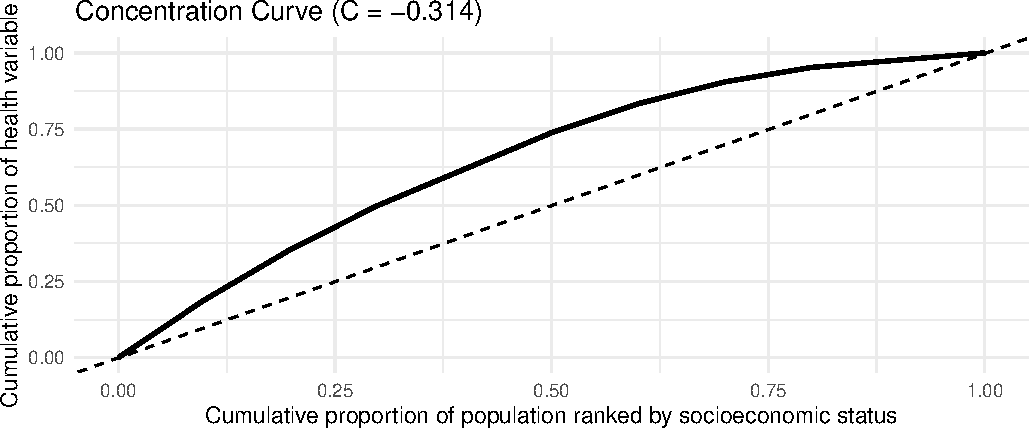
\includegraphics[keepaspectratio]{MSE_Thesis_Decomposition_of_CI_Trees_MM_files/figure-pdf/fig-concentration-curve-1.pdf}}

}

\caption{\label{fig-concentration-curve}Illustration of a concentration
curve using a simple hypothetical example.}

\end{figure}%

\subsubsection{Decomposing Socioeconomic Inequality in
Health}\label{sec-decomposing-inequality}

Inequality is measured in the observed health outcome \(y_i\), but
interventions usually work through the factors that affect health rather
than through the outcome itself. Decomposition helps relate inequality
in \(y_i\) to the observed social determinants that may explain it.

Let the health outcome for the individual \(i\) be defined.

\[
y_i = f(x_i) + \varepsilon_i,
\]

where \(x_i\) denotes the observed determinants and \(\varepsilon_i\)
represents the part that the model does not explain. Let
\(\hat{y}_i = f(x_i)\) be the fitted value, and use this fitted model to
decompose the concentration index. \[
C = \frac{2}{n\mu}\sum_{i=1}^{n} \hat{y}_i R_i - 1,
\]

where:

\(\hat{y}_i\) is the estimated health outcome for an individual \(i\)
based on the observed determinants \(x_i\).
(\citeproc{ref-wagstaff2003decomposing}{{Wagstaff, van Doorslaer and
Watanabe}, 2003}) showed that the decomposition of the concentration
index results in the following expressions: \[
C = \sum_k \left( \frac{\beta_k \bar{x}_k}{\mu} \right) C_k + \frac{GC_\varepsilon}{\mu}.
\]

In this expression, \(C\) is the concentration index of the health
outcome, \(\mu\) is the mean of that outcome, \(\beta_k\) is the
regression coefficient for determinant \(x_k\), \(\bar{x}_k\) is the
mean of \(x_k\), and \(C_k\) is the concentration index of that
determinant. The last term, \(GC_\varepsilon\), is the generalised
concentration index of the regression residuals. From this, we can infer
that the contribution to the determinant \(x_k\) is

\[
\text{Contribution of } x_k = \left( \frac{\beta_k \bar{x}_k}{\mu} \right) C_k.
\]

The concentration index(\(C_k\)) for determinant \(x_k\) can be written
as follows \[
C_k = \frac{2}{n\bar{x}_k}\sum_{i=1}^{n}x_{ki}R_i - 1.
\]

where \(x_{ki}\) is the value of determinant \(x_k\) for the individual
\(i\), \(\bar{x}_k\) is the mean of determinant \(x_k\), and \(R_i\) is
the fractional socioeconomic rank of individual \(i\).

\subsubsection{Percentage
Contributions}\label{sec-percentage-contributions}

In the concentration index results, the percentage contribution for each
determinant is usually reported. For determinant \(k\), the total
contribution is

\[
\text{AC}_k = \left(\frac{\beta_k \bar{x}_k}{\mu}\right)C_k.
\]

The percentage contribution is

\[
\text{PC}_k = 100 \times \frac{\text{AC}_k}{C}.
\]

This is a signed share of total socioeconomic inequality. In our
analysis of under-5 mortality, a positive value means that the
determinant contributes in the same direction as the observed mortality
inequality (reinforces the observed pattern). A negative value means
that it offsets part of that inequality. A percentage can exceed 100 per
cent when other determinants, or the residual term, contribute in the
opposite direction.

\subsubsection{Concentration Index Variants and a Level-Dependent
Alternative}\label{sec-ci-extensions}

When the outcome is bounded, for instance, in our case, a binary
outcome, (\citeproc{ref-wagstaff2005bounds}{Wagstaff, 2005}) showed that
the lower and upper bounds depend on the outcome's mean, so the feasible
range narrows as the mean increases. That means a change in the index
can reflect not only changes in socioeconomic inequality but also
changes in the average level of the outcome.
(\citeproc{ref-erreygers2009correcting}{Erreygers, 2009}) shows that
this issue goes beyond the binary case. In general, once a health
variable has a finite upper bound or a positive lower bound, the bounds
of the concentration index vary with the mean. For this reason, several
related measures have been introduced, rather than relying solely on the
standard index. In this thesis, the rank-dependent measures are the
standard concentration index (\(CI\)), the generalised concentration
index (\(CIg\)), and the corrected concentration index for bounded
outcomes (\(CIc\)). A level-dependent alternative, denoted \(L\), is
also considered, which is important when a socioeconomic variable has a
defensible level interpretation
(\citeproc{ref-erreygers2017socioeconomic}{Erreygers and Kessels,
2017}), for example, income.

The standard concentration index is

\[
CI_y = \frac{2}{\mu_y}\operatorname{cov}_w(y_i, R_i),
\]

where \(y_i\) is the health outcome, \(R_i\) is the fractional
socioeconomic rank, and \(\mu_y\) is the mean of the outcome.

The generalised concentration index is

\[
CIg_y = 2\operatorname{cov}_w(y_i, R_i) = \mu_y CI_y.
\]

For bounded outcomes, the corrected concentration index takes the form.

\[
CIc_y = \frac{4}{b-a}CIg_y
= \frac{8}{b-a}\operatorname{cov}_w(y_i, R_i),
\]

where \(a\) and \(b\) are the lower and upper bounds of the outcome. For
a binary outcome, where \(a=0\) and \(b=1\), this reduces to

\[
CIc_y = 4\mu_y CI_y.
\]

The level-dependent index \(L\) uses observed socioeconomic levels
directly rather than converting them into ranks:

\[
L_y =
\sum_{i=1}^{n} p_i
\left(\frac{s_i-\mu_s}{\mu_s}\right)y_i,
\qquad
p_i = \frac{w_i}{\sum_{j=1}^{n} w_j},
\qquad
\mu_s = \sum_{i=1}^{n} p_i s_i.
\]

\(s_i\) is the observed socioeconomic level, \(y_i\) is the health
outcome, and \(w_i\) is the case weight. Unlike \(CI\), \(CIg\), and
\(CIc\), the \(L\) index does not replace \(s_i\) with a fractional
rank.

The DHS wealth variable used in this thesis is the continuous
wealth-index factor score, \(v191\). It is not observed income,
consumption, or expenditure, but a PCA-derived composite measure of
household living standard based on asset ownership, housing materials,
water access, sanitation facilities, and related household amenities
(\citeproc{ref-dhsprogram_wealth_index_construction}{The DHS Program,
2007}). For the \(L\) index
(\citeproc{ref-erreygers2017socioeconomic}{Erreygers and Kessels,
2017}), state that the level-dependent construction is acceptable only
when the socioeconomic variable has ratio-scale properties; since the
wealth index is a PCA score rather than income or consumption, results
based on \(L\) should therefore be interpreted with caution. When the
concentration indeces are used as impurity measures, the tree may not
form the same subgroups under all concentration indices. A split chosen
under \(CI\) may differ from one chosen under \(CIg\), \(CIc\), or
\(L\), because each index defines inequality in a slightly different
way.

\subsubsection{Limits of the Linear
Framework}\label{sec-linear-framework-limits}

The standard decomposition uses a generalised linear model,
\(y_i = \beta_0 + \sum_k \beta_k x_{ki} + \varepsilon_i\), where
\(\beta_0\) is the intercept, \(\beta_k\) is the coefficient associated
with determinant \(x_k\), \(x_{ki}\) is the value of determinant \(k\)
for individual \(i\), and \(\varepsilon_i\) is the error term.

In the regression-based decomposition framework, each determinant
contributes through a fitted regression coefficient
(\citeproc{ref-wagstaff2003decomposing}{{Wagstaff, van Doorslaer and
Watanabe}, 2003}; \citeproc{ref-speybroeck2010decomposing}{Speybroeck
\emph{et al.}, 2010}). This makes the decomposition clear, because the
contribution of each variable can be written as part of an additive
summary. The limitation is that the coefficient is an estimated
conditional average effect over the population. The effect of a
determinant may differ by household conditions, province, maternal
background, or access to services. Some effects may also appear only
after a threshold is crossed. This is why this thesis next turns to
tree-based methods, which can represent thresholds and interactions more
directly without specifying this before fitting a model.

\subsection{Tree-Based Models for Inequality
Analysis}\label{sec-tree-based-models}

\subsubsection{Recursive Partitioning and Decision
Trees}\label{sec-recursive-partitioning-decision-trees}

A decision tree does not fit a single global equation to all
observations per determinant. It divides the data into subgroups using a
sequence of rules based on the predictors
(\citeproc{ref-hastie2009elements}{Hastie, Tibshirani and Friedman,
2017}). Each path through the tree leads to a terminal node, or leaf,
which represents a subgroup of observations with similar values on the
variables used for splitting.

In a regression tree, the fitted value for a leaf is the mean outcome in
that subgroup. In a classification tree, it is usually a class label or
an estimated class probability. The model is therefore piecewise: it
gives different summaries for different parts of the covariate space. If
the terminal regions are denoted by \(R_1,\dots,R_M\), the fitted
regression tree can be written as

\[
\hat{f}(x) = \sum_{m=1}^{M} c_m I(x \in R_m),
\]

where \(c_m\) is the fitted value assigned to region \(R_m\) and
\(I(x \in R_m)\) equals 1 if observation \(x\) falls in that region and
0 otherwise. Below Figure~\ref{fig-dhs-cart-regions} is an illustration
drawn from the Democratic Republic of the Congo (DRC) household survey
data. We fit a classification tree to predict the probability of
under-five mortality using two continuous predictors: the child's age in
months and the household wealth index. The left panel shows the tree
itself. The right panel shows the same fitted tree as a partition of the
two-dimensional predictor space. Each rectangle corresponds to one
terminal node, and all observations inside the same rectangle receive
the same fitted probability of mortality.

\begin{figure}[H]

\centering{

\pandocbounded{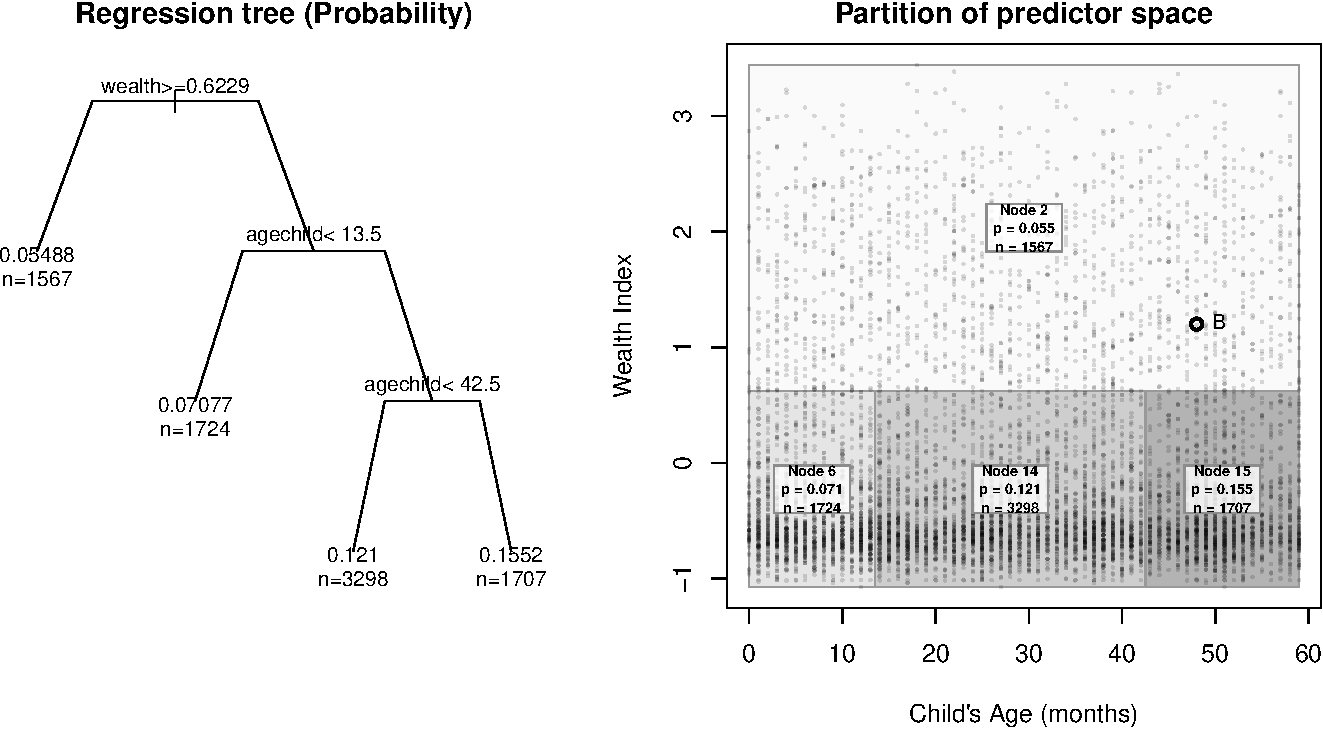
\includegraphics[keepaspectratio]{MSE_Thesis_Decomposition_of_CI_Trees_MM_files/figure-pdf/fig-dhs-cart-regions-1.pdf}}

}

\caption{\label{fig-dhs-cart-regions}A classification tree predicting
under-five mortality and its rectangular partition of (Age, Wealth)}

\end{figure}%

From the example above Figure~\ref{fig-dhs-cart-regions}, we can see the
main difference from the regression decomposition. A linear model
assigns each determinant a single coefficient, and we must specify
interactions beforehand. The same conditional average
effect(coefficient) is used for the whole sample. A tree first splits
the data into subgroups and then assigns fitted values to each subgroup.
The relationship between the outcome and the determinants can therefore
change from one part of the population to another. A decision tree thus
becomes useful when the pattern depends on thresholds, interactions, or
subgroup-specific effects.

\subsubsection{Recursive Partitioning for Inequality
Analysis}\label{sec-recursive-partitioning-inequality}

In a usual CART(Classification and Regression
Trees)(\citeproc{ref-breiman1984classification}{Breiman \emph{et al.},
1984}), splits are chosen mainly for prediction. A regression tree
searches for splits that reduce within-node outcome variation, while a
classification tree searches for splits that improve class separation
(\citeproc{ref-hastie2009elements}{Hastie, Tibshirani and Friedman,
2017}).

In this thesis, the split target is changed. The tree is used to form
subgroups where under-five mortality is less concentrated by
socioeconomic position. The outcome level in each subgroup is still
reported, but it is not the quantity used to choose the split. A split
is preferred when it reduces the within-node concentration index of
under-five mortality.

\subsubsection{Concentration-Index-Based Recursive
Partitioning}\label{sec-ci-recursive-partitioning}

To implement recursive partitioning using concentration indices, we
developed a greedy concentration-index tree. The procedure follows the
CART method of recursive partitioning but replaces the prediction
impurity with a concentration-index impurity. The gain function selects
both the variable and the split point. At node \(t\), the selected split
is

\[
(j^*, s^*)
=
\arg\max_{j \in \mathcal{J}_t,\; s \in \mathcal{S}_{jt}}
G_m(j, s, t),
\]

where \(m\) is one of \(CI\), \(CIg\), or \(CIc\), \(\mathcal{J}_t\) is
the set of candidate variables at node \(t\), and \(\mathcal{S}_{jt}\)
is the set of admissible splits for variable \(j\). The implementation
uses partykit tree representation
(\citeproc{ref-hothorn2015partykit}{Hothorn and Zeileis, 2015}).
However, it replaces the conditional-inference tree-growing engine with
a custom recursive builder whose split rule directly maximises
concentration-index gain over candidate variables and split points.

\paragraph{Weighted Within-Node Rank
Function}\label{sec-weighted-within-node-rank}

The concentration index requires individuals to be ranked from poorest
to richest. Because the tree is recursive, this ranking must be
recomputed at each node. We define a weighted within-node rank function.
For individual \(i\) belonging to node \(t\), let the weighted
fractional rank be

\[
R_{i|t}
=
\frac{1}{W_t}
\left(
\sum_{j \in t: S_j < S_i} w_j + \frac{w_i}{2}
\right),
\]

where \(S_i\) denotes the socioeconomic ranking value of individual
\(i\), and \(S_j\) denotes the corresponding value for individual \(j\)
in the same node. The terms \(w_i\) and \(w_j\) are their survey
weights, and \(W_t = \sum_{i \in t} w_i\) is the total survey weight in
node \(t\).

In this formula, the first term counts the survey weight of children in
the same node who are poorer than child \(i\), and adding half of
\(w_i\) places the child at the midpoint of its own weighted position in
the ordered list. The rank is then divided by the total node weight, so
\(R_{i|t}\) lies between 0 and 1. Since this calculation is repeated
separately inside each node, the wealth rank used by the concentration
index is local to the subgroup being split, not to the full DHS sample.

\paragraph{Node Impurity Based on the Concentration
Index}\label{sec-node-impurity-ci}

After we define within-node rank, the tree needs a criterion for
comparing possible splits. In ordinary CART, node impurity is based on
the homogeneity of the outcomes. A regression tree favours splits that
reduce within-node variance or residual sum of squares, while a
classification tree may use classification error, Gini impurity, or
entropy (\citeproc{ref-hastie2009elements}{Hastie, Tibshirani and
Friedman, 2017}). A good split should leave the two child nodes less
mixed in the outcome than the parent node. In this thesis, the same node
impurity logic is used, but the impurity measure is replaced by one
based on the concentration index.

In the present method, the aim is not to make nodes homogeneous in their
outcome level, but to make them more homogeneous with respect to
socioeconomic inequality in the outcome. We therefore define the
impurity of a node as the absolute concentration index within that node.
For node \(t\), let

\[
CI_t = \frac{2}{W_t \mu_t} \sum_{i \in t} w_i Y_i R_{i|t} - 1
\]

where

\[
\mu_t = \frac{1}{W_t}\sum_{i \in t} w_i Y_i
\]

is the weighted mean of the health outcome in node \(t\). This may be
written in weighted covariance form as

\[
CI_t = \frac{2}{\mu_t}\operatorname{cov}_w(Y_i, R_{i|t}).
\]

The quantity \(CI_t\) measures whether the health outcome is
concentrated among poorer or richer individuals within the node. Values
close to zero indicate little socioeconomic inequality within the
subgroup, while larger absolute values indicate stronger inequality.
Because the split criterion is intended to measure the strength of
inequality remaining within a node, regardless of whether it is pro-poor
or pro-rich, we use the absolute value as the impurity measure:

\[
I(t) = |CI_t|.
\]

\paragraph{Split Gain Function}\label{sec-split-gain}

At this stage, the tree needs an objective function: a rule for deciding
which split is best. At each node, the objective searches for candidate
splits and keeps the one that yields the largest improvement under the
chosen criterion.

In this thesis, the same search over candidate splits used in
classification and regression trees (CART)is retained, but the objective
function is changed. The split is not selected because it gives the best
prediction of under-five mortality in the usual trees. It is selected
because it gives the largest reduction in socioeconomic inequality in
under-five mortality.

We therefore define node impurity as the absolute value of the chosen
concentration-index measure within that node. A split is preferred when
the two child nodes contain less within-node socioeconomic inequality in
mortality than the parent node. For a candidate variable-split pair
\((j,s)\) that divides node \(t\) into a left child node \(t_L(j,s)\)
and a right child node \(t_R(j,s)\), the weighted reduction in impurity
is defined as

\[
G_m(j, s, t)
=
I_m(t)
-
\left(
\frac{W_{t_L(j,s)}}{W_t} I_m(t_L(j,s))
+
\frac{W_{t_R(j,s)}}{W_t} I_m(t_R(j,s))
\right).
\]

\(I_m(t)\) is the concentration-index impurity in the parent node, while
\(I_m(t_L(j,s))\) and \(I_m(t_R(j,s))\) are the impurities in the two
child nodes created by split \((j,s)\).

In this implementation, the gain from a split is the reduction in
weighted absolute concentration-index impurity from the parent node to
the two child nodes. If a split sends observations into two groups where
the weighted child concentration indices are closer to zero than the
parent value, the split receives a positive gain. The tree, therefore,
grows by selecting variables that reduce within-node socioeconomic
inequality, rather than by selecting variables that minimise prediction
error. After the split, the resulting child nodes can be compared by
their outcome levels and remaining inequality. Since \(I_m(t)\) is fixed
for a given parent node, maximising \(G_m(j,s,t)\) is the same as
choosing the variable-split pair that leaves the least weighted
inequality in the child nodes. The selected split is

\[
(j^*, s^*)
=
\arg\max_{j \in \mathcal{J}_t,\; s \in \mathcal{S}_{jt}}
G_m(j, s, t).
\]

The selected split is the candidate pair \((j,s)\) with the largest
admissible gain.

\paragraph{Split behaviour under alternative concentration-based
impurity measures}\label{sec-split-behaviour-impurity}

The impurity measure is not separate from the gain function. It enters
directly into the definition of the gain. Once an impurity measure has
been chosen, the gain function uses that measure to compare and rank all
admissible candidate splits at the current node.

For a candidate split \((j,s)\) at node \(t\), the gain under impurity
measure \(m\) is

\[
G_m(j,s,t)
=
I_m(t)
-
\left[
p_L I_m(t_L) + p_R I_m(t_R)
\right],
\]

where \(I_m(t)\) is the impurity of the parent node, and \(I_m(t_L)\)
and \(I_m(t_R)\) are the impurities of the left and right child nodes,
the terms \(p_L\) and \(p_R\) weight the child-node impurities by their
survey-weighted node sizes.

At a fixed parent node, \(I_m(t)\) is the same for all candidate splits
evaluated under the same impurity measure. Therefore, maximising the
gain is equivalent to minimising the weighted impurity left in the child
nodes:

\[
p_L I_m(t_L) + p_R I_m(t_R).
\]

Thus, the impurity measure affects the gain function, which in turn
ranks candidate splits. The concentration indices here are impurity
measures that are intended to be reduced. Under the standard
concentration index rule, the child-node impurity is relative to the
child-node mean:

\[
p_L \frac{A_{t_L}}{\mu_{t_L}}
+
p_R \frac{A_{t_R}}{\mu_{t_R}}.
\]

Under the generalised concentration index rule, the criterion remains on
the absolute scale:

\[
p_L A_{t_L} + p_R A_{t_R}.
\]

Because the child-node means \(\mu_{t_L}\) and \(\mu_{t_R}\) can vary
across candidate splits, the \(CI\) and \(CIg\) rules may rank the same
splits differently. The corrected concentration index \(CIc\) is
different in scale but not in ordering when the outcome range \([a,b]\)
is fixed, since

\[
G_{CIc}(j,s,t)
=
\frac{4}{b-a}G_{CIg}(j,s,t).
\]

\(\frac{4}{b-a}\) is positive and independent of the candidate split.
Therefore, \(CIc\) and \(CIg\) may produce the same split ranking,
although a fixed minimum-gain threshold would need to be rescaled if the
stopping rule uses the raw gain value.

In short, the impurity measure determines what the gain function
measures and the scale, and the gain function determines which split is
selected.

\paragraph{Split Search for Numeric and Categorical
Predictors}\label{sec-split-search}

At each node, the algorithm searches across the candidate predictors and
their admissible binary partitions. The same gain function is used for
both numeric and categorical predictors, but the candidate splits are
constructed differently. For a numeric predictor \(X_k\), the values
observed in node \(t\) are sorted, and possible cutpoints are placed
only between distinct adjacent values. For two adjacent ordered values,
\(x_{(r)}\) and \(x_{(r+1)}\), the candidate cutpoint is placed halfway
between them:

\[
s = \frac{x_{(r)} + x_{(r+1)}}{2}.
\]

This gives the binary rule.

\[
X_k \leq s
\qquad \text{versus} \qquad
X_k > s.
\]

Only cutpoints that leave enough survey weight in both child nodes are
retained. For each numeric predictor, the best admissible cutpoint is
the one with the largest concentration-index gain:

\[
s_k^* = \arg\max_s G_m(k,s,t).
\]

For a categorical predictor \(X_k\), the levels present in node \(t\)
are first ordered by their weighted mean outcome. If these ordered
levels are \(l_1,\dots,l_J\), the candidate splits are formed
cumulatively:

\[
\{l_1\} \quad \text{versus} \quad \{l_2,\dots,l_J\},
\]

\[
\{l_1,l_2\} \quad \text{versus} \quad \{l_3,\dots,l_J\},
\]

up to

\[
\{l_1,\dots,l_{J-1}\} \quad \text{versus} \quad \{l_J\}.
\]

The eligible splits are subject to the stopping rules discussed in the
next section.

\paragraph{Stopping Rules}\label{sec-stopping-rules}

A node is split only if it passes the node level checks, has at least
one admissible candidate split, and the best candidate gives enough
improvement. First, node \(t\) is searched only when its depth is below
the maximum tree depth (maxdepth), and its weighted sample size is at
least the minimum weighted parent-node size (minsplit):

\[
d_t < d_{\max}
\quad \text{and} \quad
W_t \geq W_{\mathrm{minsplit}}.
\]

If either condition fails, the node is terminal. For a node that passes
maxdepth and minsplit checks, each candidate split \((j,s)\) must create
two child nodes that are large enough. A split is admissible only if
both children satisfy the minimum weighted child-node size (minbucket),

\[
W_{t_L(j,s)} \geq W_{\mathrm{minbucket}},
\quad
W_{t_R(j,s)} \geq W_{\mathrm{minbucket}},
\]

and the minimum child-node weight proportion (minprob),

\[
\frac{W_{t_L(j,s)}}{W_t} \geq p_{\min},
\quad
\frac{W_{t_R(j,s)}}{W_t} \geq p_{\min}.
\]

These two rules remove unsuitable candidate splits before the gain is
compared. A node becomes terminal if no candidate split remains after
this filtering. Among the admissible splits, the selected split must
have a finite gain and must exceed the minimum absolute gain
(min\_gain):

\[
G_m(j^*,s^*,t) > G_{\mathrm{min}}.
\]

The algorithm also checks the minimum relative gain
(min\_relative\_gain). For split \((j,s)\), this is defined as

\[
RG_m(j,s,t)
=
\frac{G_m(j,s,t)}{|I_m(t)|}.
\]

This expresses the gain as a share of the impurity in the parent node.
It helps avoid splits that have a positive raw gain but reduce only a
very small part of the parent-node impurity. It also makes the stopping
rule less dependent on the numerical scale of the chosen
concentration-index impurity measure. Thus, a node becomes terminal when
the node-level checks fail, when no split satisfies the child-size
rules, or when the best admissible split fails the absolute or relative
gain requirement. The number of predictors considered (mtry) only
changes which predictors are searched at a node, especially in the
forest setting. It is not a stopping rule. The full algorithm is shown
in \hyperref[app-greedy-ci-tree-flow]{pseudocode} and flowchart form in
the appendix (Figure~\ref{fig-greedy-ci-tree-flow}), and the
implementation is available in the ineqTrees package
(\citeproc{ref-ineqTrees}{Mburu, 2026}).

\subsubsection{Extensions to Ensemble Methods: Random
Forests}\label{sec-random-forests}

The main advantage of the concentration-index tree is that the subgroup
structure can be inspected directly. Observed covariates define each
branch, and each terminal node can be described by its weighted sample
size, mean outcome, and remaining concentration-index value.

A limitation of the single tree is that its structure can be unstable.
The algorithm grows the tree greedily, so an early split determines
which observations are available for later splits. A small change in the
data or in the tuning controls can therefore change the upper part of
the tree and lead to a different set of terminal nodes. Tree depth also
matters. A shallow tree may miss important combinations of determinants,
while a deeper tree may start to follow small weighted subgroups rather
than a pattern that is likely to appear again in another sample.

To reduce this dependence on one fitted tree, we extend the
concentration-index split rule to a random forest. The forest fits many
greedy CI trees to perturbed versions of the training data. Within each
tree, node splitting follows the same direct maximisation of
concentration-index gain over admissible variable-split pairs used by
the \hyperref[sec-algorithmic-summary]{single-concentration-index tree}.
Randomness enters through row perturbation and, optionally, through
mtry, the number of candidate predictors searched at each node. The
final prediction is obtained by aggregating predictions across trees.

The forest contains \(B\) trees, and \(\hat{f}_b(x)\) is the prediction
from tree \(b\), the forest prediction is

\[
\hat{f}_{RF}(x) = \frac{1}{B} \sum_{b=1}^{B} \hat{f}_b(x).
\]

The interpretation of \(\hat{f}_{RF}(x)\) follows from how the forest is
fitted. Since the trees are grown to reduce concentration-index
impurity, not to minimise prediction error, we do not read the forest
output as a fully calibrated probability of under-five death. It is a
mortality-scale score obtained by averaging terminal-node mortality
values across many inequality-based trees. We use it to describe the
subgroup structure learned by the forest, not as the main target of a
predictive risk model.

Averaging over many such inequality-oriented trees makes the fitted
values less dependent on any single partition. It allows the model to
reflect more complex combinations of child, maternal, household, and
geographic characteristics. The cost is that the final forest is no
longer explainable. To address unexplainability, we fit a surrogate tree
(\citeproc{ref-dicastro2019surrogate_tree_visualization}{Di Castro and
Bertini, 2019}) to summarise the forest. The surrogate tree uses the
forest prediction \(\hat{f}_{RF}(x_i)\) as its outcome, with the same
candidate predictors used in the main analysis. It does not replace the
forest. Its role is to give a smaller set of rules that approximates the
main subgroup structure learned by the forest. The terminal nodes of
this surrogate tree can then be described using their average
forest-predicted mortality risk and their concentration index. This
gives a readable summary of how the forest separates children into
inequality-relevant groups, while keeping the random forest as the more
flexible model.

\subsubsection{Evaluation and Model Selection of Tree-Based Methods for
Inequality Analysis}\label{sec-model-selection}

The purpose of the inequality tree is to split the sample into subgroups
where under-five mortality is no longer strongly concentrated by
socioeconomic position. In an ideal terminal node, the selected
inequality index would be close to zero. Model selection, therefore,
evaluates how much of the root-node impurity is removed after
partitioning, and how much impurity remains inside the terminal nodes.
For a fitted tree, the remaining impurity is summarised by the weighted
terminal-node impurity:

\[
\sum_{\ell \in \mathcal{L}}
\frac{W_\ell}{W} I_m(D_\ell).
\]

Here \(\mathcal{L}\) is the set of terminal nodes, \(W_\ell/W\) is the
share of total survey weight in terminal node \(\ell\), and
\(I_m(D_\ell)\) is the selected node impurity. For \(CI\), \(CIg\), and
\(CIc\), \(I_m(D \ell)\) is the absolute value of the selected
concentration index. For the level-dependent measure,
\(I_L(D_\ell)=|L(D_\ell)|\). Lower values mean that the terminal nodes
are closer to the target of zero within-node socioeconomic inequality.

The stopping rules introduced earlier are treated as hyperparameters.
Cross-validation is used to select settings that yield a high gain
score. For validation, we use the held-out inequality gain:

\[
G_m^{val}(c,v)
=
I_m(D_v)
-
\sum_{\ell \in \mathcal{L}_c}
\frac{W_{\ell v}}{W_v} I_m(D_{\ell v}).
\]

\(I_m(D_v)\) is the impurity of the validation fold before splitting.
The summation is the impurity remaining after the validation
observations are dropped from the fitted tree. If \(G_m^{val}(c,v)\) is
close to absolute root inequality, the tree has reduced the validity
on-fold impurity compared with the root node. If it is close to zero,
the split structure has added a little. If it is negative, the tree has
not transferred well to the held-out fold. We also scale this gain by
the validation-fold root impurity:

\[
RG_m^{val}(c,v)
=
\frac{G_m^{val}(c,v)}{I_m(D_v)}.
\]

where \(c\) is the tunning setting being evaluated, \(v\) is the
validation fold, and \(I_m(D_v)\) is the impurity of the validation fold
before splitting. This gives the proportion of root impurity removed by
the fitted partition. For each impurity criterion, we choose the tuning
setting with the highest average relative validation gain:

\[
\overline{RG}_m^{val}(c)
=
\frac{1}{V}
\sum_{v=1}^{V} RG_m^{val}(c,v),
\]

\[
c^*
=
\arg\max_{c \in \mathcal{C}}
\overline{RG}_m^{val}(c).
\]

Raw validation shows the reduction in the original scale of the chosen
impurity measure. Training gain metrics are useful to judge overfitting.
That is when there is a large gap between the metric chosen on the
training set and that on the validation set.

\subsection{SHAP based Decomposition
Framework}\label{sec-tree-based-decomposition}

Tree-based models, including random forests, can provide flexible
predictions of health risk. This makes it hard to use them for
decomposition, since the current decomposition methods rely on
GLMs(\citeproc{ref-wagstaff2003decomposing}{{Wagstaff, van Doorslaer and
Watanabe}, 2003}; \citeproc{ref-speybroeck2010decomposing}{Speybroeck
\emph{et al.}, 2010}). To deal with this, this thesis uses SHAP values
to rewrite the fitted predictions as a sum of feature-specific
contributions.

\subsubsection{General Notation and Setup}\label{sec-decomp-setup}

We start with a dataset containing \(n\) individuals, indexed by
\(i = 1, \dots, n\). For each individual, we observe:

\begin{itemize}
\tightlist
\item
  \(y_i\), the health outcome
\item
  \(x_i = (x_{1i}, x_{2i}, \dots, x_{Ki})\), a vector of \(K\)
  determinants
\item
  \(SES_i\), a measure of socioeconomic status
\item
  \(R_i\), the fractional socioeconomic rank, defined from the most
  disadvantaged to the most advantaged using \(SES_i\)
\end{itemize}

Let \(\hat{f}(x)\) denote a fitted tree-based model, such as a random
forest. The fitted outcome for individual \(i\) is

\[
\hat{y}_i = \hat{f}(x_i).
\]

The aim is to decompose the concentration index of the fitted outcomes.
Let \(\mu_{\hat{y}}\) be the sample mean of \(\hat{y}_i\). Then the
concentration index of the fitted values is

\[
C_{\hat{y}} = \frac{2}{n\mu_{\hat{y}}}\sum_{i=1}^{n} \hat{y}_i R_i - 1.
\]

where \(C_{\hat{y}}\) is the concentration index of the fitted outcomes,
\(n\) is the sample size, and \(R_i\) is the fractional socioeconomic
rank of individual \(i\). To obtain a decomposition, we need to express
\(\hat{y}_i\) as a sum of feature-specific components.

\subsubsection{Tree-Based Predictions}\label{sec-tree-predictions}

In the regression based decomposition, the fitted value from the
regression model can be separated into terms linked to the individual
determinants. This makes the decomposition step relatively direct. The
tree models do not have that form. A child's fitted mortality risk is
determined by the path it follows through the tree and by the terminal
node it reaches. In the random forest, the fitted value is an average
over many such paths.

\subsubsection{SHAP as the Additive Link}\label{sec-shap-additive-link}

The tree and forest give fitted mortality rates, but those values are
not estimated using determinant-level coefficients. We use SHAP values
for this step. SHAP rewrites a model prediction as a baseline value plus
feature contributions (\citeproc{ref-lundberg2017unified}{Lundberg and
Lee, 2017}; \citeproc{ref-lundberg2018tree}{Lundberg, Erion and Lee,
2018}). For tree ensembles, TreeSHAP provides an efficient way to
compute these contributions.

For child \(i\), we write the fitted value as:

\[
\hat{y}_i = \phi_0 + \sum_{k=1}^{K} \phi_{ik},
\]

where \(\phi_0\) is the baseline fitted value and \(\phi_{ik}\) is the
SHAP contribution of determinant \(k\) for child \(i\). In this thesis,
\(\phi_0\) is set to the sample mean of the fitted values,
\(\mu_{\hat{y}}\). This gives the additive form needed for the next
step: the tree-based fitted value can be inserted into the
concentration-index decomposition through determinant-level SHAP
contributions.

\subsubsection{A SHAP-Based Definition of
Decomposition}\label{sec-shap-decomposition-definition}

Since we have now expressed the predictions using SHAP, we can
substitute this representation into the concentration index formula for
the predicted outcome. We start with the fractional rank \(R_i\) and the
mean prediction \(\mu_{\hat{y}} = \frac{1}{n}\sum_{i=1}^n \hat{y}_i\),
the sample concentration index of the predictions is given by:

\[
C_{\hat{y}} = \frac{2}{n\mu_{\hat{y}}}\sum_{i=1}^n \hat{y}_i R_i - 1.
\]

Recognising the property of the standard fractional rank that

\[
\sum_{i=1}^n \left(R_i - \frac{1}{2}\right)=0,
\]

We can rewrite the concentration index formula using the centred rank
\((R_i - \frac{1}{2})\). This allows us to drop the \(-1\) term. A full
proof is given in \hyperref[app-centered-rank-proof]{Appendix A}.

\[
C_{\hat{y}} = \frac{2}{n\mu_{\hat{y}}}\sum_{i=1}^n \hat{y}_i \left(R_i - \frac{1}{2}\right).
\]

We now substitute the model-level SHAP identity
\(\hat{y}_i = \phi_0 + \sum_{k=1}^K \phi_{ik}\) into this centered
formula:

\[
C_{\hat{y}} = \frac{2}{n\mu_{\hat{y}}} \sum_{i=1}^n \left( \phi_0 + \sum_{k=1}^K \phi_{ik} \right) \left(R_i - \frac{1}{2}\right).
\]

Expanding the expression yields:

\[
C_{\hat{y}} = \frac{2}{n\mu_{\hat{y}}} \left[ \phi_0 \sum_{i=1}^n \left(R_i - \frac{1}{2}\right) + \sum_{k=1}^K \sum_{i=1}^n \phi_{ik}\left(R_i - \frac{1}{2}\right) \right].
\]

Because the centred ranks sum to zero, the baseline prediction term
\(\phi_0\) cancels out:

From this point, the concentration index of the predicted outcome
simplifies to: \[
C_{\hat{y}} = \frac{2}{n\mu_{\hat{y}}} \sum_{k=1}^K \sum_{i=1}^n \phi_{ik} \left(R_i - \frac{1}{2}\right).
\]

By swapping the order of summation, we isolate the deterministic
components:

\[
C_{\hat{y}} = \sum_{k=1}^K \left[ \frac{2}{n\mu_{\hat{y}}} \sum_{i=1}^n \phi_{ik} \left(R_i - \frac{1}{2}\right) \right].
\]

We define the bracketed term as the SHAP-based inequality contribution
of feature \(k\), denoted as \(D_k^{\text{SHAP}}\):

\[
D_k^{\text{SHAP}} = \frac{2}{n\mu_{\hat{y}}} \sum_{i=1}^n \phi_{ik} \left(R_i - \frac{1}{2}\right).
\]

This results in a direct, additive SHAP decomposition for the
concentration index of the predicted outcome:

\[
C_{\hat{y}} = \sum_{k=1}^K D_k^{\text{SHAP}}.
\]

This equation shows that the absolute contribution of feature \(k\) to
health inequality is the rank-weighted average of its local SHAP
contributions, scaled by the mean predicted outcome. A feature
contributes a large share to overall inequality when its SHAP values are
large in magnitude and systematically concentrated among richer or
poorer individuals.

\subsubsection{Percentage
Contributions}\label{sec-shap-percentage-contributions}

As in \hyperref[sec-percentage-contributions]{Percentage Contributions
for decomposition based on Regression Models}, I express the SHAP-based
contributions as percentages of the concentration index for the fitted
mortality risks. For determinant \(k\), this is

\[
\text{PC}_k^{\text{SHAP}} = 100 \times \frac{D_k^{\text{SHAP}}}{C_{\hat{y}}}.
\]

In this case, \(D_k^{\text{SHAP}}\) is the absolute inequality
contribution from the SHAP values for determinant \(k\), and
\(C_{\hat{y}}\) is the concentration index of the fitted under-five
mortality risks. A positive percentage means that the determinant
contributes in the same direction as the overall predicted inequality. A
negative percentage means that it offsets part of that inequality. If
the SHAP additivity gap is small and \(C_{\hat{y}} \neq 0\), the
percentages should add up to about 100 per cent.

\subsubsection{Comparison with the Linear Decomposition
Logic}\label{sec-linear-decomposition-comparison}

The SHAP-based decomposition plays the same role as the Wagstaff
decomposition, but it uses a different object inside the contribution
term. In the regression-based framework, the absolute contribution of
determinant \(k\) is

\[
\left( \frac{\beta_k \bar{x}_k}{\mu} \right) C_k.
\]

This combines the fitted regression coefficient with the socioeconomic
distribution of the determinant. The limitation is that \(\beta_k\) is
one conditional average association for the full sample. For example, a
variable such as rural residence is treated with a single coefficient,
even though its role in under-five mortality may differ across
provinces, household conditions, and access to services. In the
tree-based decomposition, this single coefficient is replaced by
individual SHAP contributions. The absolute contribution becomes

\[
D_k^{\text{SHAP}}
=
\frac{2}{n\mu_{\hat{y}}}
\sum_{i=1}^n
\phi_{ik}
\left(R_i - \frac{1}{2}\right).
\]

Here, the contribution depends on how the SHAP value for determinant
\(k\) varies across the socioeconomic ranking. This allows the role of a
determinant to differ across children and subgroups. If rural residence
matters more in some provinces than in others, or only when combined
with other household disadvantages, that pattern is carried by the
individual values \(\phi_{ik}\) rather than by a single global
coefficient. The SHAP decomposition applies to the model-fitted outcome,
so it decomposes \(C_{\hat{y}}\) rather than \(C_y\). The observed
outcome can still be written as the fitted value plus a residual:

\[
y_i = \hat{y}_i + e_i.
\]

Using this identity, the concentration index of the observed outcome can
be separated into the inequality explained by the fitted values and the
inequality left in the residuals:

\[
C_y
=
\frac{\mu_{\hat{y}}}{\mu_y} C_{\hat{y}}
+
\frac{2}{n\mu_y}
\sum_{i=1}^n
e_i
\left(R_i - \frac{1}{2}\right).
\]

where \(C_y\) is the concentration index of the observed outcome,
\(C_{\hat{y}}\) is the concentration index of the fitted values,
\(\mu_y\) and \(\mu_{\hat{y}}\) are their means, and
\(e_i = y_i - \hat{y}_i\). The second term is the residual inequality
not captured by the fitted tree-based model.

\subsubsection{Equivalence under
Linearity}\label{sec-equivalence-linearity}

Next we test whether SHAP decomposition extension safely reduces to the
classical linear framework when the underlying model is structurally
linear, we consider a linear regression model:

\[
\hat{y}_i = \hat{\beta}_0 + \sum_{k=1}^K \hat{\beta}_k x_{ki}.
\]

According to the mathematical properties of Shapley values, under a
purely linear data-generating process, the SHAP value for a given
feature \(k\) and individual \(i\) perfectly simplifies to the estimated
coefficient multiplied by the mean-centred covariate
(\citeproc{ref-lundberg2017unified}{Lundberg and Lee, 2017})

\[
\phi_{ik} = \hat{\beta}_k (x_{ki} - \bar{x}_k).
\]

also, the baseline SHAP value \(\phi_0\) defaults exactly to the sample
mean of the predictions, \(\mu_{\hat{y}}\).

Substitute this linear SHAP identity back into our proposed tree-based
decomposition formula for the absolute contribution:

\[
D_k^{\text{SHAP}} = \frac{2}{n\mu_{\hat{y}}} \sum_{i=1}^n \phi_{ik} \left(R_i - \frac{1}{2}\right).
\]

\[
D_k^{\text{SHAP}} = \frac{2}{n\mu_{\hat{y}}} \sum_{i=1}^n \left[ \hat{\beta}_k (x_{ki} - \bar{x}_k) \right] \left(R_i - \frac{1}{2}\right).
\]

Because \(\bar{x}_k\) is a constant and
\(\sum_{i=1}^n (R_i - \frac{1}{2}) = 0\), the mean-centering term drops
out of the summation:

\[
D_k^{\text{SHAP}} = \hat{\beta}_k \left[ \frac{2}{n\mu_{\hat{y}}} \sum_{i=1}^n x_{ki} \left(R_i - \frac{1}{2}\right) \right].
\]

By definition, the concentration index of determinant \(k\) is
\(C_k = \frac{2}{n\bar{x}_k}\sum_{i=1}^{n} x_{ki}(R_i - \frac{1}{2})\).
Multiplying and dividing by \(\bar{x}_k\), we rewrite the bracketed
term:

\[
D_k^{\text{SHAP}} = \hat{\beta}_k \left( \frac{\bar{x}_k}{\mu_{\hat{y}}} \right) C_k.
\]

This is identical to the Wagstaff contribution
formula(\citeproc{ref-wagstaff2003decomposing}{{Wagstaff, van Doorslaer
and Watanabe}, 2003};
\citeproc{ref-speybroeck2010decomposing}{Speybroeck \emph{et al.},
2010}). This means the SHAP-based decomposition generalises the standard
approach, retaining equivalence under linearity while expanding to
accommodate tree ensembles.

\subsection{Simulation}\label{sec-simulation-study}

We ran a small simulation study to check whether the algorithm behaved
as expected. We first generated covariates: residence, maternal
education, and province. Then, we produced two datasets. The null data
set and the positive control. This was determined by wealth and under-5
mortality distribution. In the null case, wealth and mortality were
generated randomly. In the positive case, the planted structure
comprised three variables: residence, maternal education, and province.
Rural children formed the main at-risk group. Within this group,
children in Kasai and Nord-Kivu formed a higher-risk subgroup compared
with those in Kinshasa and Kongo Central. Children with no maternal
education formed the highest-risk subgroup. These planted groups were
assigned lower wealth and higher under-five mortality risk, with the
strongest increase among poorer children in the highest-risk subgroup.

\subsection{Analysis}\label{sec-analysis-methods}

We divided the analysis into direct and indirect decomposition methods.
The direct methods use concentration-index trees and forests, developed
here, in which the model is built to reduce socioeconomic inequality in
under-five mortality at each split. In these methods, the subgroup
structure is part of the decomposition because the tree is fitted using
the concentration-index criterion. The indirect methods first fit a
model for under-five mortality and then decompose the fitted mortality
pattern across the socioeconomic ranking.

For the regression-based indirect decomposition, we fitted a
survey-weighted logistic regression with a quasibinomial family using
the survey R package (\citeproc{ref-survey2026}{Lumley, 2026}). The
model was fitted using the DHS survey design object, including the
sampling weights and the available clustering and stratification
variables. This allowed the regression model to account for the DHS
sampling design when estimating the association between under-five
mortality and the observed child, maternal, household, occupational, and
regional determinants. We then used the margins R package to obtain
average marginal effects from the fitted survey-weighted model
(\citeproc{ref-margins2024}{Thomas J. Leeper, 2024}). These average
marginal effects express the average change in predicted under-five
mortality associated with each determinant on the response scale. We
then passed these marginal effects, together with the model matrix, the
DHS wealth ranking variable, the under-five mortality outcome, and the
sampling weights, into the Rineq R package to compute the
concentration-index decomposition
(\citeproc{ref-wagstaff2003decomposing}{{Wagstaff, van Doorslaer and
Watanabe}, 2003}; \citeproc{ref-speybroeck2010decomposing}{Speybroeck
\emph{et al.}, 2010}; \citeproc{ref-rineq2025}{Devleesschauwer \emph{et
al.}, 2025}).

The second indirect method is the
\hyperref[sec-shap-decomposition-definition]{SHAP-based decomposition}.
For this method, we fitted a predictive random forest using the
tidymodels R package with the ranger R package as the modelling backend
(\citeproc{ref-wright2017ranger}{Wright and Ziegler, 2017};
\citeproc{ref-tidymodels2020}{Kuhn and Wickham, 2020}). Because
under-five deaths were rare relative to surviving children, the alive
class was undersampled during model fitting to reduce class imbalance.
The resulting forest was therefore used as a predictive scoring model
rather than as a calibrated probability model. We then used the shapr R
package to estimate SHAP contributions from the fitted forest
(\citeproc{ref-jullum2025shapr}{Jullum \emph{et al.}, 2025}). The SHAP
analysis was used to describe how the fitted forest used the predictors,
not to estimate causal or population-level contributions of predictors
to under-five mortality.

We also fitted a comparison concentration-index tree using the rpart R
package with a custom concentration-index splitting method
(\citeproc{ref-rpart2026}{Therneau and Atkinson, 2026}). The comparison
used the same outcome, socioeconomic ranking variable, and analysis
weights as the main concentration-index tree. Node impurity was also
defined using the absolute concentration index. The main difference was
in the tree-growing tools. In the main implementation, we used custom
tree-growing controls and the partykit R package for tree representation
and plotting (\citeproc{ref-hothorn2015partykit}{Hothorn and Zeileis,
2015}). A split was accepted only if it satisfied the concentration
index tree stopping rules described in the
\hyperref[sec-stopping-rules]{tree the tree stopping rules section}. In
the rpart comparison, split search and stopping were controlled via
rpart controls, primarily minsplit, minbucket, and the complexity
parameter cp.~

For the concentration-index trees and forests, validation folds were
created at the DHS primary sampling unit level. All children from the
same PSU were kept in the same fold. The model was fitted on the
training PSUs and then evaluated on held-out PSUs using the same
validation-gain measure. This was done because children in the same
survey cluster may share local conditions and should not be treated as
fully independent observations during validation. This follows the idea
of blocked cross-validation for structured data
(\citeproc{ref-roberts2017crossvalidation}{Roberts \emph{et al.},
2017}). We report the training gain, validation gain, relative
validation gain, and tree size for the selected setting. We performed a
stability check of gain and relative gain using a bootstrap. All
children from the sampled PSUs were retained, and the tree was refitted
using the selected tuning settings using sampling with replacement. The
bootstrap results were used to describe how often the same split
variables and similar terminal-node structures were recovered, not as a
formal replicate-weight survey inference procedure. Tree similarity was
measured using Jaccard overlap between terminal-node memberships in the
selected tree and the bootstrap-refitted tree. A higher Jaccard value
means that the two trees placed more of the same children into
comparable terminal subgroups.

\section{Results}\label{results}

\subsection{Exploratory Data Analysis}\label{exploratory-data-analysis}

In the DRC Data Set(\citeproc{ref-dhs_drc_2007_dataset}{The DRC Program
Program, 2007}), 10.32\% of children died before reaching age five
(Figure~\ref{fig-results-wealth-distribution}). Deaths were more
commonly observed among children from disadvantaged or rural
backgrounds. The children who died differed descriptively from those who
survived. Low-wealth households accounted for a larger share of deaths
than of survivors (51.3\% versus 42.8\%). The same pattern was present
for rural residence (69.3\% versus 60.7\%), no skilled attendance at
birth (65.6\% versus 56.8\%), and mothers with no education (67.5\%
versus 55.2\%) (Table~\ref{tbl-appendix-weighted-baseline}). Mortality
also differed across provinces, ranging from 6.2\% in Kinshasa to 14.2\%
in Katanga (Figure~\ref{fig-appendix-province-mortality-distribution}).
Next we use the direct and indirect methods for decomposition.

\begin{figure}[H]

\centering{

\pandocbounded{
\includegraphics[keepaspectratio]{MSE_Thesis_Decomposition_of_CI_Trees_MM_files/figure-pdf/fig-results-wealth-distribution-1.pdf}}

}

\caption{\label{fig-results-wealth-distribution}Under-five mortality
distribution and DHS wealth index in the DRC analysis data.}

\end{figure}%

\subsection{Decomposition of determinants of under-five
mortality}\label{decomposition-of-determinants-of-under-five-mortality}

\subsubsection{Indirect methods comparison (regression and
predictive-forest
SHAP)}\label{indirect-methods-comparison-regression-and-predictive-forest-shap}

From the indirect decomposition, the largest CI regression contribution
was mother's education, followed by father's occupation in agriculture,
mother's occupation in agriculture, household wealth, residence, and
skilled birth attendance (Table~\ref{tbl-results-method-comparison}). In
the predictive-forest SHAP decomposition, the contributions were less
concentrated in the education and occupation variables. Residence gave
the largest SHAP contribution under CI, CIg, CIc, and L. Under CI, CIg,
and CIc, residence contributed about 19\%, followed by father's
agricultural occupation, household wealth, mother's education, Maniema,
mother's agricultural occupation, and skilled birth attendance. Under L,
residence was again the largest contributor, followed by father's
agricultural occupation, mother's education, Maniema, mother's
agricultural occupation, Kinshasa, and household wealth. The fitted
regression model is reported in
Table~\ref{tbl-appendix-regression-model-summary}. Details of the fitted
predictive forest are provided in
Table~\ref{tbl-appendix-ranger-sampling-summary} and
Table~\ref{tbl-appendix-ranger-cross-validation}, and its SHAP
contributions are shown in Figure~\ref{fig-appendix-shap-summary}.

\begingroup\fontsize{11}{13}\selectfont

\begin{longtable}{>{\raggedright\arraybackslash}p{4.4cm}>{\raggedleft\arraybackslash}p{1.35cm}>{\raggedleft\arraybackslash}p{1.35cm}>{\raggedleft\arraybackslash}p{1.35cm}>{\raggedleft\arraybackslash}p{1.35cm}>{\raggedleft\arraybackslash}p{1.35cm}>{\raggedleft\arraybackslash}p{1.35cm}>{\raggedleft\arraybackslash}p{1.35cm}}

\caption{\label{tbl-results-method-comparison}Regression and
predictive-forest SHAP percentage contributions by criterion.}

\tabularnewline

\toprule
\multicolumn{1}{c}{\textbf{ }} & \multicolumn{3}{c}{\textbf{Regression}} & \multicolumn{4}{c}{\textbf{Predictive-forest SHAP}} \\
\cmidrule(l{3pt}r{3pt}){2-4} \cmidrule(l{3pt}r{3pt}){5-8}
\textbf{Variable} & \textbf{CI (\%)} & \textbf{CIg (\%)} & \textbf{CIc (\%)} & \textbf{CI (\%)} & \textbf{CIg (\%)} & \textbf{CIc (\%)} & \textbf{L (\%)}\\
\midrule
Mother's education & 31.232 & 170.974 & 170.974 & 8.101 & 8.101 & 8.101 & 9.518\\
Father's occupation: Agriculture & 24.119 & 117.979 & 117.979 & 8.537 & 8.537 & 8.537 & 9.633\\
Mother's occupation: Agriculture & 16.135 & 87.330 & 87.330 & 6.864 & 6.864 & 6.864 & 6.730\\
Household wealth & 12.699 & 53.789 & 53.789 & 8.335 & 8.335 & 8.335 & 6.155\\
Type of residence & 12.019 & 71.760 & 71.760 & 19.418 & 19.418 & 19.418 & 23.992\\
\addlinespace
Skilled birth attendance & 10.741 & 60.069 & 60.069 & 6.415 & 6.415 & 6.415 & 1.362\\
Region: Equateur & 5.118 & 6.371 & 6.371 & 4.116 & 4.116 & 4.116 & 3.327\\
Father's occupation: Household, unskilled, not working & -4.569 & -5.692 & -5.692 & -0.667 & -0.667 & -0.667 & -1.049\\
Region: Kinshasa & -4.102 & -3.621 & -3.621 & 3.204 & 3.204 & 3.204 & 6.102\\
Region: Sud-Kivu & -2.783 & -1.299 & -1.299 & -3.520 & -3.520 & -3.520 & -4.137\\
\addlinespace
Region: Kasai Oriental & -2.287 & -2.951 & -2.951 & 1.548 & 1.548 & 1.548 & 1.192\\
Father's education & -2.023 & -5.285 & -5.285 & 2.185 & 2.185 & 2.185 & 3.424\\
Region: Maniema & 1.604 & 0.547 & 0.547 & 7.644 & 7.644 & 7.644 & 8.955\\
Region: Orientale & -1.174 & -1.314 & -1.314 & -0.545 & -0.545 & -0.545 & -0.377\\
Birth order and interval: 5+ short interval & -0.998 & -0.985 & -0.985 & -0.105 & -0.105 & -0.105 & 4.641\\
\addlinespace
Region: Bas-Congo & -0.926 & -0.360 & -0.360 & 0.535 & 0.535 & 0.535 & 0.749\\
Mother's occupation: Household, unskilled, not working & 0.778 & 1.749 & 1.749 & -0.748 & -0.748 & -0.748 & -1.236\\
Region: Kasai Occidental & 0.629 & 0.648 & 0.648 & -0.821 & -0.821 & -0.821 & -0.259\\
Birth order and interval: 5+ long interval & -0.615 & -1.565 & -1.565 & -1.987 & -1.987 & -1.987 & -2.629\\
Sex of the child & -0.581 & -2.775 & -2.775 & -1.638 & -1.638 & -1.638 & 0.343\\
\addlinespace
Region: Katanga & -0.447 & -0.446 & -0.446 & 2.125 & 2.125 & 2.125 & 2.451\\
Mother's age at birth & 0.364 & 1.522 & 1.522 & 0.651 & 0.651 & 0.651 & -1.015\\
Region: Nord-Kivu & 0.233 & 0.088 & 0.088 & 1.128 & 1.128 & 1.128 & 1.094\\
Birth order and interval: 2-4 long interval & 0.208 & 0.685 & 0.685 & -1.104 & -1.104 & -1.104 & -2.907\\
Birth order and interval: 2-4 short interval & -0.006 & -0.006 & -0.006 & -6.310 & -6.310 & -6.310 & -6.461\\
\bottomrule

\end{longtable}

\endgroup{}

\subsection{Direct methods (concentration-index trees and
forests)}\label{direct-methods-concentration-index-trees-and-forests}

\subsubsection{Rank Dependent Concentration-Index
Tree}\label{rank-dependent-concentration-index-tree}

\paragraph{\texorpdfstring{The Corrected Concentration-Index Tree
\(CIc\)}{The Corrected Concentration-Index Tree CIc}}\label{the-corrected-concentration-index-tree-cic}

We start with a tree based on the corrected concentration index,
appropriate for bounded outcomes
(\citeproc{ref-erreygers2009correcting}{Erreygers, 2009}). In the fitted
data, the selected \(CIc\) tree shows that inequality in under-five
mortality is structured mainly through maternal education, father's
agricultural occupation, skilled birth attendance, household wealth, and
residence in Katanga Figure~\ref{fig-appendix-ci-tree-cic}. The first
separation is by maternal education. Among children whose mothers had
some education, the tree then separates the father's agricultural
occupation and skilled birth attendance. Among children whose mothers
had no education, the tree separates household wealth and then Katanga.
The lowest-mortality terminal group consists of children whose mothers
had some education and whose fathers were not in agriculture, with an
under-five mortality rate of about 6.5\%. The highest-mortality terminal
group consists of children whose mothers had no education, who lived in
low-wealth households, and who resided in Katanga, with a mortality of
about 17.8\%.

\begin{figure}[H]

\centering{

\pandocbounded{
\includegraphics[keepaspectratio]{MSE_Thesis_Decomposition_of_CI_Trees_MM_files/figure-pdf/fig-appendix-ci-tree-cic-1.pdf}}

}

\caption{\label{fig-appendix-ci-tree-cic}Concentration-index tree fitted
with the CIc criterion.}

\end{figure}%

\paragraph{\texorpdfstring{Generalised and standard concentration-index
trees \(CIg\) and
\(CI\)}{Generalised and standard concentration-index trees CIg and CI}}\label{generalised-and-standard-concentration-index-trees-cig-and-ci}

The appendix also shows the trees fitted using the generalised and
standard concentration indices. The generalised concentration-index tree
gives the same fitted subgroup structure as the corrected
concentration-index tree Figure~\ref{fig-appendix-ci-tree-cig}. The
mortality pattern is therefore substantively unchanged.

The standard concentration-index tree gives a closely related structure,
but it adds one further split among children whose mothers had some
education and whose fathers were not in agriculture
Figure~\ref{fig-appendix-ci-tree-ci}. In this branch, children without a
short preceding birth interval have the lowest mortality, about 6.0\%,
while children with a short preceding birth interval have a mortality of
about 11.7\%. Apart from this additional demographic distinction, the
standard \(CI\) tree points to the same main sources of inequality as
the corrected and generalised trees: maternal education, father's
agricultural occupation, skilled birth attendance, household wealth, and
residence in Katanga.

\subsubsection{\texorpdfstring{Level dependent Concentration-Index Tree
\(L\)}{Level dependent Concentration-Index Tree L}}\label{level-dependent-concentration-index-tree-l}

We then fit a tree based on the level-dependent concentration index
criterion, \(L\) (\citeproc{ref-erreygers2017socioeconomic}{Erreygers
and Kessels, 2017}). This index is most appropriate when the
socioeconomic variable has ratio-scale properties. We treat it as a
sensitivity analysis; the selected \(L\) tree shows that inequality in
under-five mortality is structured primarily by rural residence,
father's agricultural occupation, household wealth, and province,
especially Kinshasa, Equateur, and Katanga
Figure~\ref{fig-results-selected-ci-tree}. The lowest-mortality terminal
group consists of urban children in Kinshasa whose fathers were not in
agriculture, with an under-five mortality rate of about 5.1\%. The
highest-mortality terminal group consists of rural children living in
low-wealth households in Katanga, with an under-five mortality rate of
about 18.5\%. Thus, the level-dependent tree tells a more spatial story
of inequality: mortality risk is first organised by the rural-urban
divide, then by occupation, wealth, and region. This structure differs
from the rank-dependent trees, which first organise the fitted subgroups
around maternal education and father's agricultural occupation.

\begin{figure}[H]

\centering{


\includegraphics[width=1\linewidth,height=\textheight,keepaspectratio]{MSE_Thesis_Decomposition_of_CI_Trees_MM_files/figure-pdf/fig-results-selected-ci-tree-1.pdf}

}

\caption{\label{fig-results-selected-ci-tree}Level dependent
concentration-index tree for under-five mortality in the DRC.}

\end{figure}%

\subsubsection{Tree validation plots}\label{tree-validation-plots}

The validation results indicated that the subgroup structure learned by
these trees during training did not generalise well to held-out samples.
The rank-dependent trees based on \(CI\), \(CIg\), and \(CIc\) gave
strong training gains, removing 83.3\% of root-node impurity for \(CI\)
and 81.6\% for both \(CIc\) and \(CIg\)
Table~\ref{tbl-appendix-tree-selected-setting-summary}. However, their
validation gains were negative under the PSU-held-out folds
Figure~\ref{fig-appendix-tree-validation-path}, Table~\ref{tbl-appendix-tree-selected-setting-summary}.
A negative validation gain indicates that the fitted terminal nodes did
not reduce the concentration-index impurity in the held-out PSUs
relative to the root node. Thus, although the rank-dependent trees
identified plausible subgroup structure in the fitted sample, the same
partitions did not generalise well to clusters not used to fit the tree.

The level-dependent \(L\) tree showed a different validation pattern. It
removed 98.2\% of root-node impurity during training. It retained a
positive validation gain of 64.5\% under the same PSU-held-out
validation criterion, so the rural-urban, occupational, wealth, and
regional partition was more reproducible across held-out clusters
Figure~\ref{fig-appendix-tree-validation-path}, Table~\ref{tbl-appendix-tree-selected-setting-summary}.
This does not make \(L\) the definitive main result, because \(L\) is
most appropriate when the socioeconomic variable has ratio-scale
properties, and the DHS wealth index is a PCA-derived asset score.

\begin{figure}[H]

\centering{

\pandocbounded{
\includegraphics[keepaspectratio]{MSE_Thesis_Decomposition_of_CI_Trees_MM_files/figure-pdf/fig-appendix-tree-validation-path-1.pdf}}

}

\caption{\label{fig-appendix-tree-validation-path}Tree validation gain
and complexity by minimum relative split gain.}

\end{figure}%

\paragraph{Tree complexity plots}\label{tree-complexity-plots}

Tree complexity decreased as the minimum relative split gain increased,
since larger thresholds allowed only splits that removed a larger share
of parent-node impurity Figure~\ref{fig-appendix-tree-complexity-path}.
The selected settings produced relatively small trees across the 10
PSU-held-out validation folds, with mean terminal-node counts of 6.9 for
\(CI\), 6.0 for \(CIc\), 6.0 for \(CIg\), and 7.5 for \(L\)
Table~\ref{tbl-appendix-tree-selection}, Figure~\ref{fig-appendix-tree-complexity-path}.
These decimal values are averages across validation-fold refits. They
should not be read as the number of terminal nodes in a single final
fitted tree, which must be an integer.

\begin{figure}[H]

\centering{

\pandocbounded{
\includegraphics[keepaspectratio]{MSE_Thesis_Decomposition_of_CI_Trees_MM_files/figure-pdf/fig-appendix-tree-complexity-path-1.pdf}}

}

\caption{\label{fig-appendix-tree-complexity-path}Tree complexity by
number of terminal nodes.}

\end{figure}%

\paragraph{Bootstrap stability of selected
trees}\label{bootstrap-stability-of-selected-trees}

\begingroup\fontsize{11}{13}\selectfont

\begin{longtable}[t]{>{\raggedright\arraybackslash}p{1.2cm}>{\raggedright\arraybackslash}p{1.6cm}>{\raggedright\arraybackslash}p{1.8cm}>{\raggedright\arraybackslash}p{4.0cm}>{\raggedright\arraybackslash}p{2.7cm}>{\raggedright\arraybackslash}p{2.7cm}}

\caption{\label{tbl-results-bootstrap-tree-stability}Bootstrap stability
of selected concentration-index trees}

\tabularnewline

\\
\toprule
\textbf{Criterion} & \textbf{No split refits} & \textbf{Terminal nodes} & \textbf{Root split} & \textbf{Relative gain} & \textbf{Tree similarity}\\
\midrule
CI & 1.0\% & 6 (2, 10) & Mother's education, 41.7\% & 0.463 (0.287, 0.767) & 0.270 (0.074, 0.683)\\
CIg & 3.0\% & 5 (1, 9) & Mother's education, 39.9\% & 0.500 (0.330, 0.789) & 0.313 (0.148, 0.758)\\
CIc & 1.8\% & 5 (2, 9) & Mother's education, 45.3\% & 0.505 (0.335, 0.800) & 0.331 (0.148, 0.761)\\
L & 0.0\% & 6 (3, 11) & Type of residence, 67.2\% & 0.930 (0.784, 0.997) & 0.277 (0.074, 0.841)\\
\bottomrule

\end{longtable}

\endgroup{}

The bootstrap stability checks resampled primary sampling units and
refitted the selected tree settings. All criteria completed 1000
successful refits with no failures. The table shows that the
rank-dependent trees most often split first on mother's education, while
the \(L\) tree most often split first on residence. The \(L\) tree had
the highest relative gain, but tree similarity remained modest across
all criteria.

\paragraph{Rpart comparison}\label{rpart-comparison}

The rpart comparison tree recovered the same upper-level structure as
the main CI tree (Figure~\ref{fig-appendix-ci-tree-ci};
Figure~\ref{fig-appendix-lecturer-rpart-robust}). Both trees first split
on maternal education, then separated children by father's agricultural
occupation among those whose mothers had some education, and by
household wealth among those whose mothers had no education. The
high-mortality branch was also similar, identifying children whose
mothers had no education, who lived in low-wealth households, and who
resided in Katanga. The main difference was in the lower branches: the
rpart comparison introduced a split by long preceding birth interval,
while the main CI tree used a short preceding birth-interval split. This
suggests that the main rank-dependent structure was not driven only by
the custom implementation, although some lower-level refinements
depended on the tree-growing and stopping rules.

\begin{figure}[H]

\centering{

\pandocbounded{
\includegraphics[keepaspectratio]{MSE_Thesis_Decomposition_of_CI_Trees_MM_files/figure-pdf/fig-appendix-lecturer-rpart-robust-1.pdf}}

}

\caption{\label{fig-appendix-lecturer-rpart-robust}Rpart comparison tree
using CI impurity.}

\end{figure}%

\subsubsection{Concentration index forest and surrogate
tree}\label{concentration-index-forest-and-surrogate-tree}

\paragraph{Forest validation plots}\label{forest-validation-plots}

We evaluated concentration-index forests using the same
impurity-reduction validation criterion as the single trees. The
selected forest settings used a minimum relative split gain of 0.20 to
0.25; larger values produced very shallow forests with mean
terminal-node counts close to the root, so they did not reveal
additional subgroup structure
Figure~\ref{fig-appendix-forest-validation-path}, Figure~\ref{fig-appendix-forest-complexity-path}.

For rank-dependent criteria, forests reduced training gains relative to
corresponding single trees but did not yield a stable validation
pattern. The \(CI\), \(CIc\), and \(CIg\) forests removed 48.1\%,
51.7\%, and 51.6\% of root-node impurity in training
Table~\ref{tbl-appendix-forest-selected-setting-summary}, Table~\ref{tbl-appendix-tree-selected-setting-summary}.
Their validation-gain ratios remained negative: -1038.3\% for \(CI\),
-1108.5\% for \(CIc\), and -1063.0\% for \(CIg\)
Figure~\ref{fig-appendix-forest-validation-path}, Table~\ref{tbl-appendix-forest-selected-setting-summary}.
Thus, averaging across trees reduced the size of the training gain, but
it did not make the rank-dependent forest partitions reproducible under
the validation criterion.

The tuning path shows the trade-off between validation performance and
complexity. As the minimum relative split gain increased, the component
trees became shallower
Figure~\ref{fig-appendix-forest-validation-path}, Figure~\ref{fig-appendix-forest-complexity-path}.
The level-dependent forest remained the most stable. It removed 95.3\%
of root-node impurity in training and retained a positive validation
gain of 56.7\% Table~\ref{tbl-appendix-forest-selected-setting-summary}.
As with the \(L\) tree, this result is interpreted as a sensitivity
analysis because the DHS wealth index is not a ratio-scale socioeconomic
variable.

\begin{figure}[H]

\centering{

\pandocbounded{
\includegraphics[keepaspectratio]{MSE_Thesis_Decomposition_of_CI_Trees_MM_files/figure-pdf/fig-appendix-forest-validation-path-1.pdf}}

}

\caption{\label{fig-appendix-forest-validation-path}Forest validation
gain and complexity by minimum relative split gain.}

\end{figure}%

\paragraph{Surrogate trees from Forest
Predictions}\label{surrogate-trees-from-forest-predictions}

To interpret the selected forest, we fitted a surrogate tree to
summarise its predictions (Figure~\ref{fig-results-surrogate-tree}). The
surrogate tree retained the main structure seen in the \(CIg\) forest.
We present the \(CIg\) surrogate because the \(CIc\) surrogate did not
identify terminal nodes with concentration-index values close to zero.

\begin{figure}[H]

\centering{

\pandocbounded{
\includegraphics[keepaspectratio]{MSE_Thesis_Decomposition_of_CI_Trees_MM_files/figure-pdf/fig-results-surrogate-tree-1.pdf}}

}

\caption{\label{fig-results-surrogate-tree}Surrogate tree for the CIg
concentration-index forest.}

\end{figure}%

The other surrogate trees can be found in the appendix
(Figure~\ref{fig-appendix-forest-surrogate-l};
Figure~\ref{fig-appendix-forest-surrogate-cic};
Figure~\ref{fig-appendix-forest-surrogate-ci}).

\subsubsection{Variable importance}\label{variable-importance}

The variable-importance plots compare the fitted \(CIc\) tree with the
\(CIg\) forest that is summarised by the displayed surrogate tree
Figure~\ref{fig-results-selected-model-variable-importance}. In the
\(CIc\) tree, the largest reductions in concentration-index impurity
come from mother's education, father's agricultural occupation,
household wealth, Katanga, and skilled birth attendance.

\begin{figure}[H]

\centering{

\pandocbounded{
\includegraphics[keepaspectratio]{MSE_Thesis_Decomposition_of_CI_Trees_MM_files/figure-pdf/fig-results-selected-model-variable-importance-1.pdf}}

}

\caption{\label{fig-results-selected-model-variable-importance}Variable
importance for the CIc concentration-index tree and CIg
concentration-index forest.}

\end{figure}%

The \(CIg\) forest gives a broader ranking than the single \(CIc\) tree.
Mother's education remains the leading variable, but the forest also
gives weight to household wealth, father's agricultural occupation,
mother's agricultural occupation, residence, and regional indicators. In
the appendix plots, the same groups of variables appear again under the
other criteria: residence, region, occupation, education, and wealth
Figure~\ref{fig-appendix-tree-variable-importance}, Figure~\ref{fig-appendix-forest-variable-importance}.

\subsection{Simulation Study}\label{simulation-study}

\subsubsection{Null case}\label{null-case}

From (Figure~\ref{fig-results-simulation-null-trees}) we see that the
algorithm developed here did not find a meaningful structure and behaved
as expected. This shows that the tree-growing rule does not create
subgroup structure when the outcome and socioeconomic ranking are
independent, since the tree uses concentraion index as an impurity
measure, which measures how sociaeconomic ranking and outcome covary.

\begin{figure}[H]

\begin{minipage}[t]{0.50\linewidth}

\centering{

\pandocbounded{
\includegraphics[keepaspectratio]{MSE_Thesis_Decomposition_of_CI_Trees_MM_files/figure-pdf/fig-results-simulation-null-trees-1.pdf}}

}

\subcaption{\label{fig-results-simulation-null-trees-1}CI}

\end{minipage}%
%
\begin{minipage}[t]{0.50\linewidth}

\centering{

\pandocbounded{
\includegraphics[keepaspectratio]{MSE_Thesis_Decomposition_of_CI_Trees_MM_files/figure-pdf/fig-results-simulation-null-trees-2.pdf}}

}

\subcaption{\label{fig-results-simulation-null-trees-2}CIg}

\end{minipage}%
\newline
\begin{minipage}[t]{0.50\linewidth}

\centering{

\pandocbounded{
\includegraphics[keepaspectratio]{MSE_Thesis_Decomposition_of_CI_Trees_MM_files/figure-pdf/fig-results-simulation-null-trees-3.pdf}}

}

\subcaption{\label{fig-results-simulation-null-trees-3}CIc}

\end{minipage}%
%
\begin{minipage}[t]{0.50\linewidth}

\centering{

\pandocbounded{
\includegraphics[keepaspectratio]{MSE_Thesis_Decomposition_of_CI_Trees_MM_files/figure-pdf/fig-results-simulation-null-trees-4.pdf}}

}

\subcaption{\label{fig-results-simulation-null-trees-4}L}

\end{minipage}%

\caption{\label{fig-results-simulation-null-trees}Null simulation
concentration-index trees by criterion.}

\end{figure}%

\subsubsection{Poor subgroup case}\label{poor-subgroup-case}

In the positive-control simulation, the method(the concentration index
tree with \(CIc\) as an impurity measure) recovered the planted subgroup
structure. The tree first separated urban from rural observations, then
split the rural group by province and maternal education
(Figure~\ref{fig-results-simulation-tree}). This structure matched the
way the simulated outcome was generated: poorer observations in the
planted rural, low-education, selected-province subgroup had higher
outcome prevalence. The terminal nodes also followed the expected
gradient, with the highest prevalence among observations in the most
disadvantaged planted subgroup.

\begin{figure}[H]

\centering{

\pandocbounded{
\includegraphics[keepaspectratio]{MSE_Thesis_Decomposition_of_CI_Trees_MM_files/figure-pdf/fig-results-simulation-tree-1.pdf}}

}

\caption{\label{fig-results-simulation-tree}CIc concentration-index tree
recovered from simulated data with a known subgroup-generating
mechanism.}

\end{figure}%

We see the same pattern across the sensitivity plots in the appendix the
trees developed using \(CI\), \(CIg\), and \(CIc\), and \(L\) as
impurity
measures(Figure~\ref{fig-appendix-simulation-positive-control-ci};
Figure~\ref{fig-appendix-simulation-positive-control-cic};
Figure~\ref{fig-appendix-simulation-positive-control-l}).

\section{Discussion}\label{discussion}

\subsection{Main findings}\label{main-findings}

This thesis developed and applied a tree-based model for analysing
socioeconomic inequality in under-five mortality using the concentration
index impurity. The main finding is that inequality in the DRC data
could not be explained by household wealth alone. Under-five mortality
was also related to residence, maternal education, skilled birth
attendance, parental occupation, and province. Overall, 10.32\% of
children died before age five. The children who died were more often
from low-wealth households, rural households, mothers with no education,
births without skilled attendance, and some provinces, especially
Katanga. This is in line with earlier DRC work on geographic variation
in under-five mortality, and with decomposition studies showing that
wealth, education, residence, and occupation contribute to mortality
inequalities in African settings
(\citeproc{ref-vanmalderen2013under5}{Van Malderen, Van Oyen and
Speybroeck, 2013}; \citeproc{ref-kandala2014drc}{Kandala \emph{et al.},
2014}; \citeproc{ref-vanmalderen2019socioeconomic}{Van Malderen \emph{et
al.}, 2019}).

The indirect methods provided a variable view of this inequality. In the
regression based decomposition, mother's education made the largest
regression contribution, followed by father's agricultural occupation,
mother's agricultural occupation, household wealth, residence, and
skilled birth attendance. These results are consistent with earlier
decomposition work, which found that household wealth, parental
education, occupation, and residence were important contributors to
under-five mortality inequality
(\citeproc{ref-vanmalderen2013under5}{Van Malderen, Van Oyen and
Speybroeck, 2013}; \citeproc{ref-vanmalderen2019socioeconomic}{Van
Malderen \emph{et al.}, 2019}). The SHAP analysis, from the fitted
random forest, gave a less concentrated picture. Residence was the
largest SHAP contributor, while household wealth, parental occupation,
mother's education, skilled birth attendance, and some regional
indicators also appeared across criteria. SHAP-based decomposition
therefore adds to the regression methods by allowing a more flexible
fitted model, such as a random forest, to be summarised at the
determinant level. These SHAP results should be read as an explanation
of the fitted predictive model rather than as causal or population-level
determinant contributions.

The direct concentration-index trees added the subgroup interpretation
that is less visible in the regression-based decomposition. While the
indirect methods ranked variables by their contribution to inequality,
the trees showed how these variables combined within the data to define
groups with different inequality patterns. The rank-dependent trees
based on \(CI\), \(CIg\), and \(CIc\) identified a structure involving
maternal education, father's agricultural occupation, skilled birth
attendance, household wealth, and Katanga. Mortality was lower among
children whose mothers had some education and whose fathers were not in
agriculture, and higher among children whose mothers had no education,
who lived in low-wealth households, and who resided in Katanga. However,
these partitions did not validate well. Although the rank-based methods
removed about 87\% to 88\% of root-node inequality in training, their
validation gains were negative, suggesting that the strong training
structure did not transfer well to held-out folds.

\subsection{Rank-dependent and level-dependent views of
inequality}\label{rank-dependent-and-level-dependent-views-of-inequality}

From these analyses, we see differences in the results
(Figure~\ref{fig-appendix-ci-tree-ci};
Figure~\ref{fig-appendix-ci-tree-cig};
Figure~\ref{fig-appendix-ci-tree-cic}) in subgroups formed by the two
ways of defining the impurity measure when developing the concentration
index tree. In the rank-dependent criteria \(CI\), \(CIg\), and \(CIc\),
a child's contribution depends on the child's position in the current
node's socioeconomic ranking. After each split, the children in the new
subgroup are ranked again, so the same child can receive a different
rank because the comparison group has changed. In the level-dependent
criterion, re-ranking is still done but in \(L\), the child's observed
socioeconomic level is carried into the subgroup, so a child's rank also
reflects their wealth level.

The differences also showed up in cross-validation; the level-dependent
method outperformed the rank-dependent methods. The rank-dependent trees
had strong training performance but negative validation gains, while the
level-dependent tree kept a positive validation gain
(Figure~\ref{fig-appendix-tree-validation-path};
Table~\ref{tbl-appendix-tree-selected-setting-summary}). The same
pattern was seen in the forests: averaging trees reduced the validation
loss for the rank-dependent criteria, but their validation gains
remained below zero, whereas the \(L\) forest retained a positive
validation gain (Figure~\ref{fig-appendix-forest-validation-path};
Table~\ref{tbl-appendix-forest-selected-setting-summary}). The
validation results show that \(CI\), \(CIg\), and \(CIc\) identified
detailed in-sample subgroup rules, whereas \(L\) produced a more
reproducible subgroup structure in this application.

These results are also mirrored by the subgroup-decomposability argument
in (\citeproc{ref-erreygers2017subgroup}{Erreygers \emph{et al.},
2017}). In their comparison of rank-dependent and level-dependent
measures, they show that the level-dependent index \(L\) is
subgroup-decomposable and rank-dependent measures are more difficult to
decompose cleanly across population groups. Decomposability of the
level-dependent concentration index shown by
(\citeproc{ref-erreygers2017subgroup}{Erreygers \emph{et al.}, 2017})
can also explain why \(L\) performed better as a tree impurity criterion
in this application: children inherit their socioeconomic level within
each subgroup, rather than being re-weighted only by a new within-node
rank. Although the DHS wealth index is an asset-based
score(\citeproc{ref-dhsprogram_wealth_index_construction}{The DHS
Program, 2007}) and (\citeproc{ref-erreygers2017socioeconomic}{Erreygers
and Kessels, 2017}) recommends using Level depedent concentration
index(\(L\)) with a wealth-ranking variable that has ratio properties.
The cross-validation results show that the \(L\) concentration index
impurity measure yielded a structure transferable to held-out samples
using the DHS wealth score.

\subsection{Methodological and data
limitations}\label{methodological-and-data-limitations}

This thesis uses DHS survey data from the Democratic Republic of the
Congo (\citeproc{ref-dhs_drc_2007_dataset}{The DRC Program Program,
2007}). The DHS Program states that participation is voluntary and that
respondents' identities and information are kept confidential
(\citeproc{ref-dhs_privacy_respondents}{The DHS Program, 2026}).
However, the data still have the usual limitations of retrospective
household surveys. Under-five mortality is reconstructed from birth
histories, so the estimates depend on correct reporting of births,
dates, and child survival status. Non-response, recall error, and
misreporting of dates may affect the mortality estimates. The survey is
also from 2007. It was useful for comparing the new method with earlier
work on the same setting. However, the results should not be read as
describing the current situation in the Democratic Republic of the
Congo.

The second limitation is the socioeconomic ranking variable. The DHS
wealth index is constructed from household assets and living-standard
variables, typically using principal component analysis
(\citeproc{ref-dhsprogram_wealth_index_construction}{The DHS Program,
2007}). It is useful for ordering households from poorer to richer, but
it is not a measure of income, consumption, or expenditure. It is also a
relative score within the survey. This limitation mainly affects the
level-dependent concentration index. For \(L\), the interpretation is
clearer when the socioeconomic variable has ratio-scale properties
(\citeproc{ref-erreygers2017socioeconomic}{Erreygers and Kessels,
2017}).

Decision trees are known to be unstable: small changes in the data can
produce different split variables, split points, and tree structures.
This comes from the recursive and greedy nature of tree construction.
Once an early split changes, all later splits are fitted to different
subsets of the data. In this thesis, this was handled partly through
cross-validation and through splitting controls such as minimum node
size, minimum child-node proportion, maximum depth, minimum gain, and
minimum relative gain. These controls helped restrict weak or very small
splits, but they do not remove the instability problem completely.

Another limitation is the use of a surrogate tree to summarise the
forest. The forest was added to reduce dependence on a single greedy
tree, but the resulting forest is harder to interpret than a single
tree. To obtain an interpretable summary, a surrogate tree was fitted
using the forest's risk estimates. The surrogate still chooses splits by
maximising concentration-index gain, but the outcome used in that split
rule is the forest-predicted risk rather than the observed mortality
outcome. This approximation of the forest, therefore, depends on the
correctness of the forest.

Another limitation comes from SHAP-based decomposition. This analysis
was based on a predictive random forest and should be interpreted as an
explanation of that fitted prediction model, not as a decomposition of
population mortality risk. SHAP values depend on the fitted model and on
the SHAP convention used. This is important in DHS data because maternal
education, occupation, residence, and household wealth are correlated.
The allocation of predictive contribution across these variables is
therefore not unique, and the SHAP results should not be interpreted as
causal or determinant contributions. The predictive forest used for the
SHAP analysis was also affected by undersampling. As shown in the
appendix, the alive class was undersampled, changing the weighted class
distribution from about 89.7\% alive and 10.3\% died to about 60.0\%
alive and 40.0\% died. Unless the predictions are recalibrated, the
fitted values from this model should be treated as prediction scores
rather than calibrated mortality probabilities. The predictive
performance of this forest was modest, with ROC AUC values around 0.61.
This does not invalidate the SHAP analysis, but it limits confidence in
detailed feature rankings. For this reason, the SHAP results are treated
as a descriptive explanation of the fitted predictive model, rather than
as evidence that the listed variables contribute those proportions to
the risk of under-five mortality.

\subsection{Ethical, societal, and stakeholder
relevance}\label{ethical-societal-and-stakeholder-relevance}

This thesis uses child-level data from the Democratic Republic of the
Congo DHS phase V survey (\citeproc{ref-dhs_drc_2007_dataset}{The DRC
Program Program, 2007}). These data contain sensitive information,
including child survival status, birth histories, household wealth,
residence, province, maternal education, occupation, and skilled birth
attendance. Even without names, the data describe mothers, children,
households, and family deaths. The DHS Program states that participation
is voluntary and that respondents' identities and information are kept
confidential (\citeproc{ref-dhs_privacy_respondents}{The DHS Program,
2026}). In this thesis, we used secondary survey data and should remain
within the conditions under which we were granted access to the DHS
files.

The concentration index trees developed here can identify subgroups with
higher mortality and greater socioeconomic disadvantage. For example,
the fitted trees point to rural children from low-wealth households in
Katanga, or children whose mothers had no education and who lived in
low-wealth households. These subgroups are useful for public health
analysis and planning, but the results should be used carefully. Groups
we identified through concentration index trees should not be described
as if the children, mothers, or provinces are the problem. The tree is
showing where mortality and disadvantage are concentrated in the data.
The interpretation should therefore focus on unequal conditions, access
to services, and policy response, not labelling groups.

Compared with GLM based decomposition, tree-based models are easier to
interpret. The variable percentage contribution from regression or
Shap-based decomposition can show which variables contribute more.
However, it cannot show how disadvantage is organised across residence,
household wealth, occupation, maternal background, and province. A tree
is easier to discuss because it works like a flow chart. As shown in
this thesis, the tree partitions the data graphically into high- and
low-risk groups. Concentration index trees make it easier to follow the
path to these high- and low-risk groups and identify them for public
health planning. This makes tree models useful in public health and
policy contexts, where the goal is to identify groups for targeted
interventions. They are also easy to interpret for non-technical groups.

\section{Future research}\label{future-research}

In this thesis, the level-dependent \(L\) method yielded more stable
validation results than the rank-dependent criteria. This suggests that
the choice of concentration index, used here as the tree impurity
measure, is an important part of the method. One useful direction for
future work would be to investigate whether rank-dependent
concentration-index trees can be modified so that a child node retains
more information about the wealth position from which its observations
came, rather than relying solely on the new within-node ranking after
each split. This may help reduce some of the instability seen in the
rank-dependent trees.

\section{Conclusion}\label{conclusion}

This thesis developed and applied a tree-based method for analysing
socioeconomic inequality in under-five mortality. The method used the
concentration index as the impurity measure in a recursive partitioning
method. Instead of ranking determinants by their percentage contribution
to inequality, the fitted tree produced subgroups that could be
interpreted as decision rules. This added a subgroup view to the usual
regression-based decomposition. In the DRC DHS application, inequality
in under-five mortality was not explained solely by household wealth.
Residence, maternal education, skilled birth attendance, parental
occupation, household wealth, and province all appeared in the analysis.

The indirect methods gave the variable-level view, while the direct
trees showed how these variables combined. The regression decomposition
emphasised the mother's education and the father's agricultural
occupation. The SHAP-based decomposition gave a broader pattern, with
residence, household wealth, mother's education, skilled birth
attendance, and parental occupation appearing across criteria.

The concentration-index trees acted as a direct method to decomposition,
which showed directly with subgroups had higher under 5 deaths
concentration. The rank-dependent trees found an
education-occupation-wealth pattern, with higher mortality among
children whose mothers had no education, who lived in low-wealth
households, and who resided in Katanga. The \(L\) method gave a more
spatial structure, beginning with residence and then splitting by
occupation, wealth, and province.

In this thesis, the level-dependent \(L\) method yielded more stable
validation results than the rank-dependent criteria. This suggests that
the choice of concentration index, used here as the tree impurity
measure, is an important part of the method. The rank-dependent trees
found detailed structures in the fitted data, but these structures did
not validate well. The \(L\) tree and forest retained positive
validation gains, so the level-dependent result was the more stable
descriptive partition in this application.

Since the level-dependent concentration index, as a measure of impurity,
produced better results on held-out folds, future research should
examine how to improve rank-dependent trees to retain more information
from the original wealth ranking after each split.

\section{References}\label{sec-references}

\protect\phantomsection\label{refs}
\begin{CSLReferences}{0}{1}
\bibitem[\citeproctext]{ref-breiman1984classification}
Breiman, L. \emph{et al.} (1984) \emph{Classification and regression
trees}. Available at: \url{https://doi.org/10.1201/9781315139470}.

\bibitem[\citeproctext]{ref-rineq2025}
Devleesschauwer, B. \emph{et al.} (2025) \emph{Rineq: Concentration
index and decomposition for health inequalities}. Available at:
\url{https://doi.org/10.32614/CRAN.package.rineq}.

\bibitem[\citeproctext]{ref-dicastro2019surrogate_tree_visualization}
Di Castro, F. and Bertini, E. (2019) {`Surrogate decision tree
visualization: Interpreting and visualizing black-box classification
models with surrogate decision tree'}, in \emph{Joint proceedings of the
ACM IUI 2019 workshops}. Los Angeles, USA (CEUR workshop proceedings),
pp. 1--5. Available at:
\url{https://ceur-ws.org/Vol-2327/IUI19WS-ExSS2019-15.pdf}.

\bibitem[\citeproctext]{ref-erreygers2009correcting}
Erreygers, G. (2009) {`Correcting the concentration index'},
\emph{Journal of Health Economics}, 28(2), pp. 504--515. Available at:
\url{https://doi.org/10.1016/j.jhealeco.2008.02.003}.

\bibitem[\citeproctext]{ref-erreygers2017subgroup}
Erreygers, G. \emph{et al.} (2017) {`Subgroup decomposability of
income-related inequality of health, with an application to australia'},
\emph{Economic Record} {[}Preprint{]}. Available at:
\url{https://doi.org/10.1111/1475-4932.12373}.

\bibitem[\citeproctext]{ref-erreygers2017socioeconomic}
Erreygers, G. and Kessels, R. (2017) {`Socioeconomic status and health:
A new approach to the measurement of bivariate inequality'},
\emph{International Journal of Environmental Research and Public
Health}, 14(7), p. 673. Available at:
\url{https://doi.org/10.3390/ijerph14070673}.

\bibitem[\citeproctext]{ref-hastie2009elements}
Hastie, T., Tibshirani, R. and Friedman, J. (2017) \emph{The elements of
statistical learning: Data mining, inference, and prediction}. 12th edn.
Springer Science \& Business Media. Available at:
\url{https://hastie.su.domains/ElemStatLearn/}.

\bibitem[\citeproctext]{ref-hothorn2015partykit}
Hothorn, T. and Zeileis, A. (2015) {`{partykit}: A modular toolkit for
recursive partytioning in {R}'}, \emph{Journal of Machine Learning
Research}, 16, pp. 3905--3909. Available at:
\url{https://jmlr.org/papers/v16/hothorn15a.html}.

\bibitem[\citeproctext]{ref-jones2003_child_survival}
Jones, G. \emph{et al.} (2003) {`How many child deaths can we prevent
this year?'}, \emph{The Lancet}, 362(9377), pp. 65--71. Available at:
\url{https://doi.org/10.1016/S0140-6736(03)13811-1}.

\bibitem[\citeproctext]{ref-jullum2025shapr}
Jullum, M. \emph{et al.} (2025) {`Shapr: Explaining machine learning
models with conditional shapley values in {R} and python'}, \emph{arXiv
preprint arXiv:2504.01842} {[}Preprint{]}. Available at:
\url{https://arxiv.org/abs/2504.01842}.

\bibitem[\citeproctext]{ref-kakwani1997socioeconomic}
{Kakwani, N., Wagstaff, A. and van Doorslaer, E.} (1997) {`Socioeconomic
inequalities in health: Measurement, computation, and statistical
inference'}, \emph{Journal of Econometrics}, 77(1), pp. 87--103.
Available at: \url{https://doi.org/10.1016/S0304-4076(96)01807-6}.

\bibitem[\citeproctext]{ref-kandala2014drc}
Kandala, N.-B. \emph{et al.} (2014) {`Child mortality in the democratic
republic of congo: Cross-sectional evidence of the effect of geographic
location and prolonged conflict from a national household survey'},
\emph{BMC Public Health}, 14(1), p. 266. Available at:
\url{https://doi.org/10.1186/1471-2458-14-266}.

\bibitem[\citeproctext]{ref-tidymodels2020}
Kuhn, M. and Wickham, H. (2020) \emph{Tidymodels: A collection of
packages for modeling and machine learning using tidyverse principles}.
Available at: \url{https://www.tidymodels.org}.

\bibitem[\citeproctext]{ref-survey2026}
Lumley, T. (2026) \emph{Survey: Analysis of complex survey samples}.

\bibitem[\citeproctext]{ref-lundberg2018tree}
Lundberg, S.M., Erion, G.G. and Lee, S.-I. (2018) {`Consistent
individualized feature attribution for tree ensembles'}, \emph{arXiv
preprint arXiv:1802.03888} {[}Preprint{]}. Available at:
\url{https://doi.org/10.48550/arXiv.1802.03888}.

\bibitem[\citeproctext]{ref-lundberg2017unified}
Lundberg, S.M. and Lee, S.-I. (2017) {`A unified approach to
interpreting model predictions'}, in \emph{Advances in neural
information processing systems}. Available at:
\url{https://doi.org/10.48550/arXiv.1705.07874}.

\bibitem[\citeproctext]{ref-ineqTrees}
Mburu, M. (2026) \emph{ineqTrees: Tree-based decomposition of health
inequality}. Available at: \url{https://github.com/m-mburu/ineqTrees}.

\bibitem[\citeproctext]{ref-roberts2017crossvalidation}
Roberts, D.R. \emph{et al.} (2017) {`Cross-validation strategies for
data with temporal, spatial, hierarchical, or phylogenetic structure'},
\emph{Ecography} {[}Preprint{]}. Available at:
\url{https://doi.org/10.1111/ecog.02881}.

\bibitem[\citeproctext]{ref-sharrow2022_under5_mortality}
{Sharrow, D. \emph{et al.}} (2022) {`Global, regional, and national
trends in under-5 mortality between 1990 and 2019 with scenario-based
projections until 2030: A systematic analysis by the UN inter-agency
group for child mortality estimation'}, \emph{The Lancet Global Health},
10(2), pp. e195--e206. Available at:
\url{https://doi.org/10.1016/S2214-109X(21)00515-5}.

\bibitem[\citeproctext]{ref-speybroeck2010decomposing}
Speybroeck, N. \emph{et al.} (2010) {`Decomposing socioeconomic health
inequalities'}, \emph{International Journal of Public Health}, 55, pp.
347--351. Available at: \url{https://doi.org/10.1007/s00038-009-0105-z}.

\bibitem[\citeproctext]{ref-dhsprogram_wealth_index_construction}
The DHS Program (2007) {`Wealth index construction'}. The DHS Program.
Available at:
\url{https://dhsprogram.com/topics/wealth-index/Wealth-Index-Construction.cfm}.

\bibitem[\citeproctext]{ref-dhs_privacy_respondents}
The DHS Program (2026) {`Protecting the privacy of DHS survey
respondents'}. Methodology webpage. Available at:
\url{https://dhsprogram.com/methodology/protecting-the-privacy-of-dhs-survey-respondents.cfm}.

\bibitem[\citeproctext]{ref-dhs_drc_2007_dataset}
The DRC Program Program (2007) {`{Congo Democratic Republic: Standard
DHS, 2007}'}. Survey dataset page. Available at:
\url{https://dhsprogram.com/methodology/survey/survey-display-239.cfm}.

\bibitem[\citeproctext]{ref-rpart2026}
Therneau, T. and Atkinson, B. (2026) \emph{Rpart: Recursive partitioning
and regression trees}. Available at:
\url{https://doi.org/10.32614/CRAN.package.rpart}.

\bibitem[\citeproctext]{ref-margins2024}
Thomas J. Leeper (2024) \emph{Margins: Marginal effects for model
objects}. Available at:
\url{https://CRAN.R-project.org/package=margins}.

\bibitem[\citeproctext]{ref-tsala_dimbuene2022_drc_health_insurance}
Tsala Dimbuene, Z., Muanza Nzuzi, R. and Nzita Kikhela, P.-D. (2022)
{`Poverty, education and health insurance coverage among women of
reproductive ages in the democratic republic of the congo: A
cross-sectional and multilevel analysis'}, \emph{BMJ Open}, 12, p.
e064834. Available at:
\url{https://doi.org/10.1136/bmjopen-2022-064834}.

\bibitem[\citeproctext]{ref-vanmalderen2019socioeconomic}
Van Malderen, C. \emph{et al.} (2019) {`Socioeconomic factors
contributing to under-five mortality in sub-saharan africa: A
decomposition analysis'}, \emph{BMC Public Health}, 19(1), p. 760.
Available at: \url{https://doi.org/10.1186/s12889-019-7111-8}.

\bibitem[\citeproctext]{ref-vanmalderen2013under5}
Van Malderen, C., Van Oyen, H. and Speybroeck, N. (2013) {`Contributing
determinants of overall and wealth-related inequality in under-5
mortality in 13 african countries'}, \emph{Journal of Epidemiology and
Community Health}, 67(8), pp. 667--676. Available at:
\url{https://doi.org/10.1136/jech-2012-202195}.

\bibitem[\citeproctext]{ref-wagstaff2005bounds}
Wagstaff, A. (2005) {`The bounds of the concentration index when the
variable of interest is binary, with an application to immunization
inequality'}, \emph{Health Economics}, 14(4), pp. 429--432. Available
at: \url{https://doi.org/10.1002/hec.953}.

\bibitem[\citeproctext]{ref-wagstaff2003decomposing}
{Wagstaff, A., van Doorslaer, E. and Watanabe, N.} (2003) {`On
decomposing the causes of health sector inequalities with an application
to malnutrition inequalities in vietnam'}, \emph{Journal of
Econometrics}, 112(1), pp. 207--223. Available at:
\url{https://doi.org/10.1016/S0304-4076(02)00161-6}.

\bibitem[\citeproctext]{ref-who_gho_under5_mortality_indicator}
World Health Organisation (2026) \emph{Child deaths: Under-five
mortality rate (per 1000 live births) (SDG 3.2.1)}. Available at:
\url{https://www.who.int/data/gho/data/indicators/indicator-details/GHO/under-five-mortality-rate-(probability-of-dying-by-age-5-per-1000-live-births)}
(Accessed: 26 April 2026).

\bibitem[\citeproctext]{ref-wright2017ranger}
Wright, M.N. and Ziegler, A. (2017) {`Ranger: A fast implementation of
random forests for high dimensional data in {C++} and {R}'},
\emph{Journal of Statistical Software}, 77(1), pp. 1--17. Available at:
\url{https://doi.org/10.18637/jss.v077.i01}.

\end{CSLReferences}

\section{Generative AI Disclosure}\label{generative-ai-disclosure}

\begin{itemize}
\tightlist
\item
  I have used ChatGPT (GenAI tool) to support the development of the
  ineqTrees package after defining the main functions and writing
  starter code.
\item
  I have used ChatGPT and Grammarly (GenAI/writing support tools) for
  English language improvement, spelling, and clarity.
\item
  I used ChatGPT to help develop custom tree plots, especially plots
  where each node displays wealth, sample size, and the outcome.
\end{itemize}

\section{Appendix}\label{sec-appendix}

\subsection{Code}\label{code}

\begin{itemize}
\tightlist
\item
  The Analysis code for this thesis is available at
  https://github.com/m-mburu/thesis-mse
\item
  The code for the concentration-index tree and forest implementation is
  available at https://github.com/m-mburu/ineqTrees
\end{itemize}

\subsection{Appendix A: Proof that the Centered Ranks Sum to
Zero}\label{app-centered-rank-proof}

This appendix provides the algebra used in
\hyperref[sec-shap-decomposition-definition]{Section 4.4}.

For the standard fractional rank,

\[
R_i = \frac{i - 0.5}{n},
\]

where \(i\) is the individual's position (from \(1\) to \(n\)) when
ordered by socioeconomic status.

If we sum this rank across all \(n\) individuals, we obtain

\[
\begin{aligned}
\sum_{i=1}^n R_i &= \frac{1}{n} \sum_{i=1}^n (i - 0.5) \\
&= \frac{1}{n} \left( \sum_{i=1}^n i - \sum_{i=1}^n 0.5 \right).
\end{aligned}
\]

Using \(\sum_{i=1}^n i = \frac{n(n+1)}{2}\) and
\(\sum_{i=1}^n 0.5 = 0.5n\), it follows that

\[
\begin{aligned}
\sum_{i=1}^n R_i &= \frac{1}{n} \left( \frac{n(n+1)}{2} - 0.5n \right) \\
&= \frac{1}{n} \left( \frac{n^2 + n - n}{2} \right) \\
&= \frac{1}{n} \left( \frac{n^2}{2} \right) \\
&= \frac{n}{2}.
\end{aligned}
\]

Therefore,

\[
\begin{aligned}
\sum_{i=1}^n \left( R_i - \frac{1}{2} \right) &= \sum_{i=1}^n R_i - \sum_{i=1}^n \frac{1}{2} \\
&= \frac{n}{2} - \left(n \times \frac{1}{2}\right) \\
&= \frac{n}{2} - \frac{n}{2} \\
&= 0.
\end{aligned}
\]

\subsection{\texorpdfstring{Appendix B: Numerical Example Comparing
\(CI\) and
\(CIg\)}{Appendix B: Numerical Example Comparing CI and CIg}}\label{app-ci-cig-example}

This appendix illustrates the result stated in
\hyperref[sec-split-behaviour-impurity]{Section 3.3.4}.

Consider two candidate splits \(s_1\) and \(s_2\) with equal child-node
weights \(p_L = p_R = \tfrac12\). Here \(A_{t_L}\) and \(A_{t_R}\)
denote the absolute generalised concentration-index components in the
left and right child nodes, while \(\mu_{t_L}\) and \(\mu_{t_R}\) are
the corresponding child-node mean outcomes.

For \(s_1\), suppose

\[
A_{t_L}=A_{t_R}=0.06,
\qquad
\mu_{t_L}=\mu_{t_R}=0.10.
\]

For \(s_2\), suppose

\[
A_{t_L}=A_{t_R}=0.08,
\qquad
\mu_{t_L}=\mu_{t_R}=0.50.
\]

Then the \(CIg\)-based child-node objective is

\[
\frac12(0.06)+\frac12(0.06)=0.06
\quad \text{for } s_1,
\]

and

\[
\frac12(0.08)+\frac12(0.08)=0.08
\quad \text{for } s_2.
\]

So \(CIg\) prefers \(s_1\).

However, the \(CI\)-based child-node objective is

\[
\frac12\left(\frac{0.06}{0.10}\right)+\frac12\left(\frac{0.06}{0.10}\right)=0.60
\quad \text{for } s_1,
\]

and

\[
\frac12\left(\frac{0.08}{0.50}\right)+\frac12\left(\frac{0.08}{0.50}\right)=0.16
\quad \text{for } s_2.
\]

So \(CI\) prefers \(s_2\). This shows that relative and absolute
inequality criteria can lead to different split choices.

\subsection{Greedy Concentration-Index Tree-Growing Procedure
Flowchart}\label{app-greedy-ci-tree-flow}

\paragraph{Algorithmic Summary}\label{algorithmic-summary}

The complete procedure we have built up to this point is summarised as
follows.

Algorithm: Concentration-index-based recursive partitioning

Input:

\begin{itemize}
\tightlist
\item
  health outcome \(Y\)
\item
  socioeconomic ranking variable \(S\)
\item
  candidate predictors \(X_1,\dots,X_p\)
\item
  survey weights \(w_i\)
\end{itemize}

At node \(t\):

\begin{enumerate}
\def\labelenumi{\arabic{enumi}.}
\tightlist
\item
  Compute the weighted within-node socioeconomic ranks \(R_{i|t}\) from
  \(S\).
\item
  Stop if maxdepth, the maximum permitted tree depth, or minsplit, the
  minimum weighted parent-node size, prevents further splitting.
\item
  Optionally sample mtry candidate predictors, where mtry is the number
  of predictors searched at a node.
\item
  For every candidate predictor \(X_j\), generate binary split
  candidates:

  \begin{itemize}
  \tightlist
  \item
    if \(X_j\) is numeric, evaluate cutpoints \(s\) between distinct
    ordered values;
  \item
    if \(X_j\) is categorical, evaluate admissible binary partitions of
    its levels, using ordered cumulative partitions where needed.
  \end{itemize}
\item
  Reject candidates that violate minbucket, the minimum weighted
  child-node size, or minprob, the minimum child-node share of the
  parent-node weight.
\item
  For every remaining candidate pair \((j,s)\), compute the
  concentration-index gain \(G_m(j,s,t)\).
\item
  Choose the split
\end{enumerate}

\[
(j^*,s^*) = \arg\max_{j,s} G_m(j,s,t).
\]

\begin{enumerate}
\def\labelenumi{\arabic{enumi}.}
\setcounter{enumi}{7}
\tightlist
\item
  Stop if the best gain is not finite, is less than or equal to
  min\_gain, or, when min\_relative\_gain is positive, does not exceed
  the required share of the parent-node impurity.
\item
  Otherwise split node \(t\) into child nodes \(t_L\) and \(t_R\), then
  repeat the procedure recursively.
\end{enumerate}

The same recursive logic is shown as a flowchart in
Figure~\ref{fig-greedy-ci-tree-flow}. The procedures are implemented in
the ineqTrees package (\citeproc{ref-ineqTrees}{Mburu, 2026}). The
fitted tree is stored using the partykit tree representation for
plotting and traversal (\citeproc{ref-hothorn2015partykit}{Hothorn and
Zeileis, 2015}).

\subsubsection{Flowchart of the Greedy Concentration-Index Tree-Growing
Procedure}\label{flowchart-of-the-greedy-concentration-index-tree-growing-procedure}

\begin{figure}[H]

\centering{

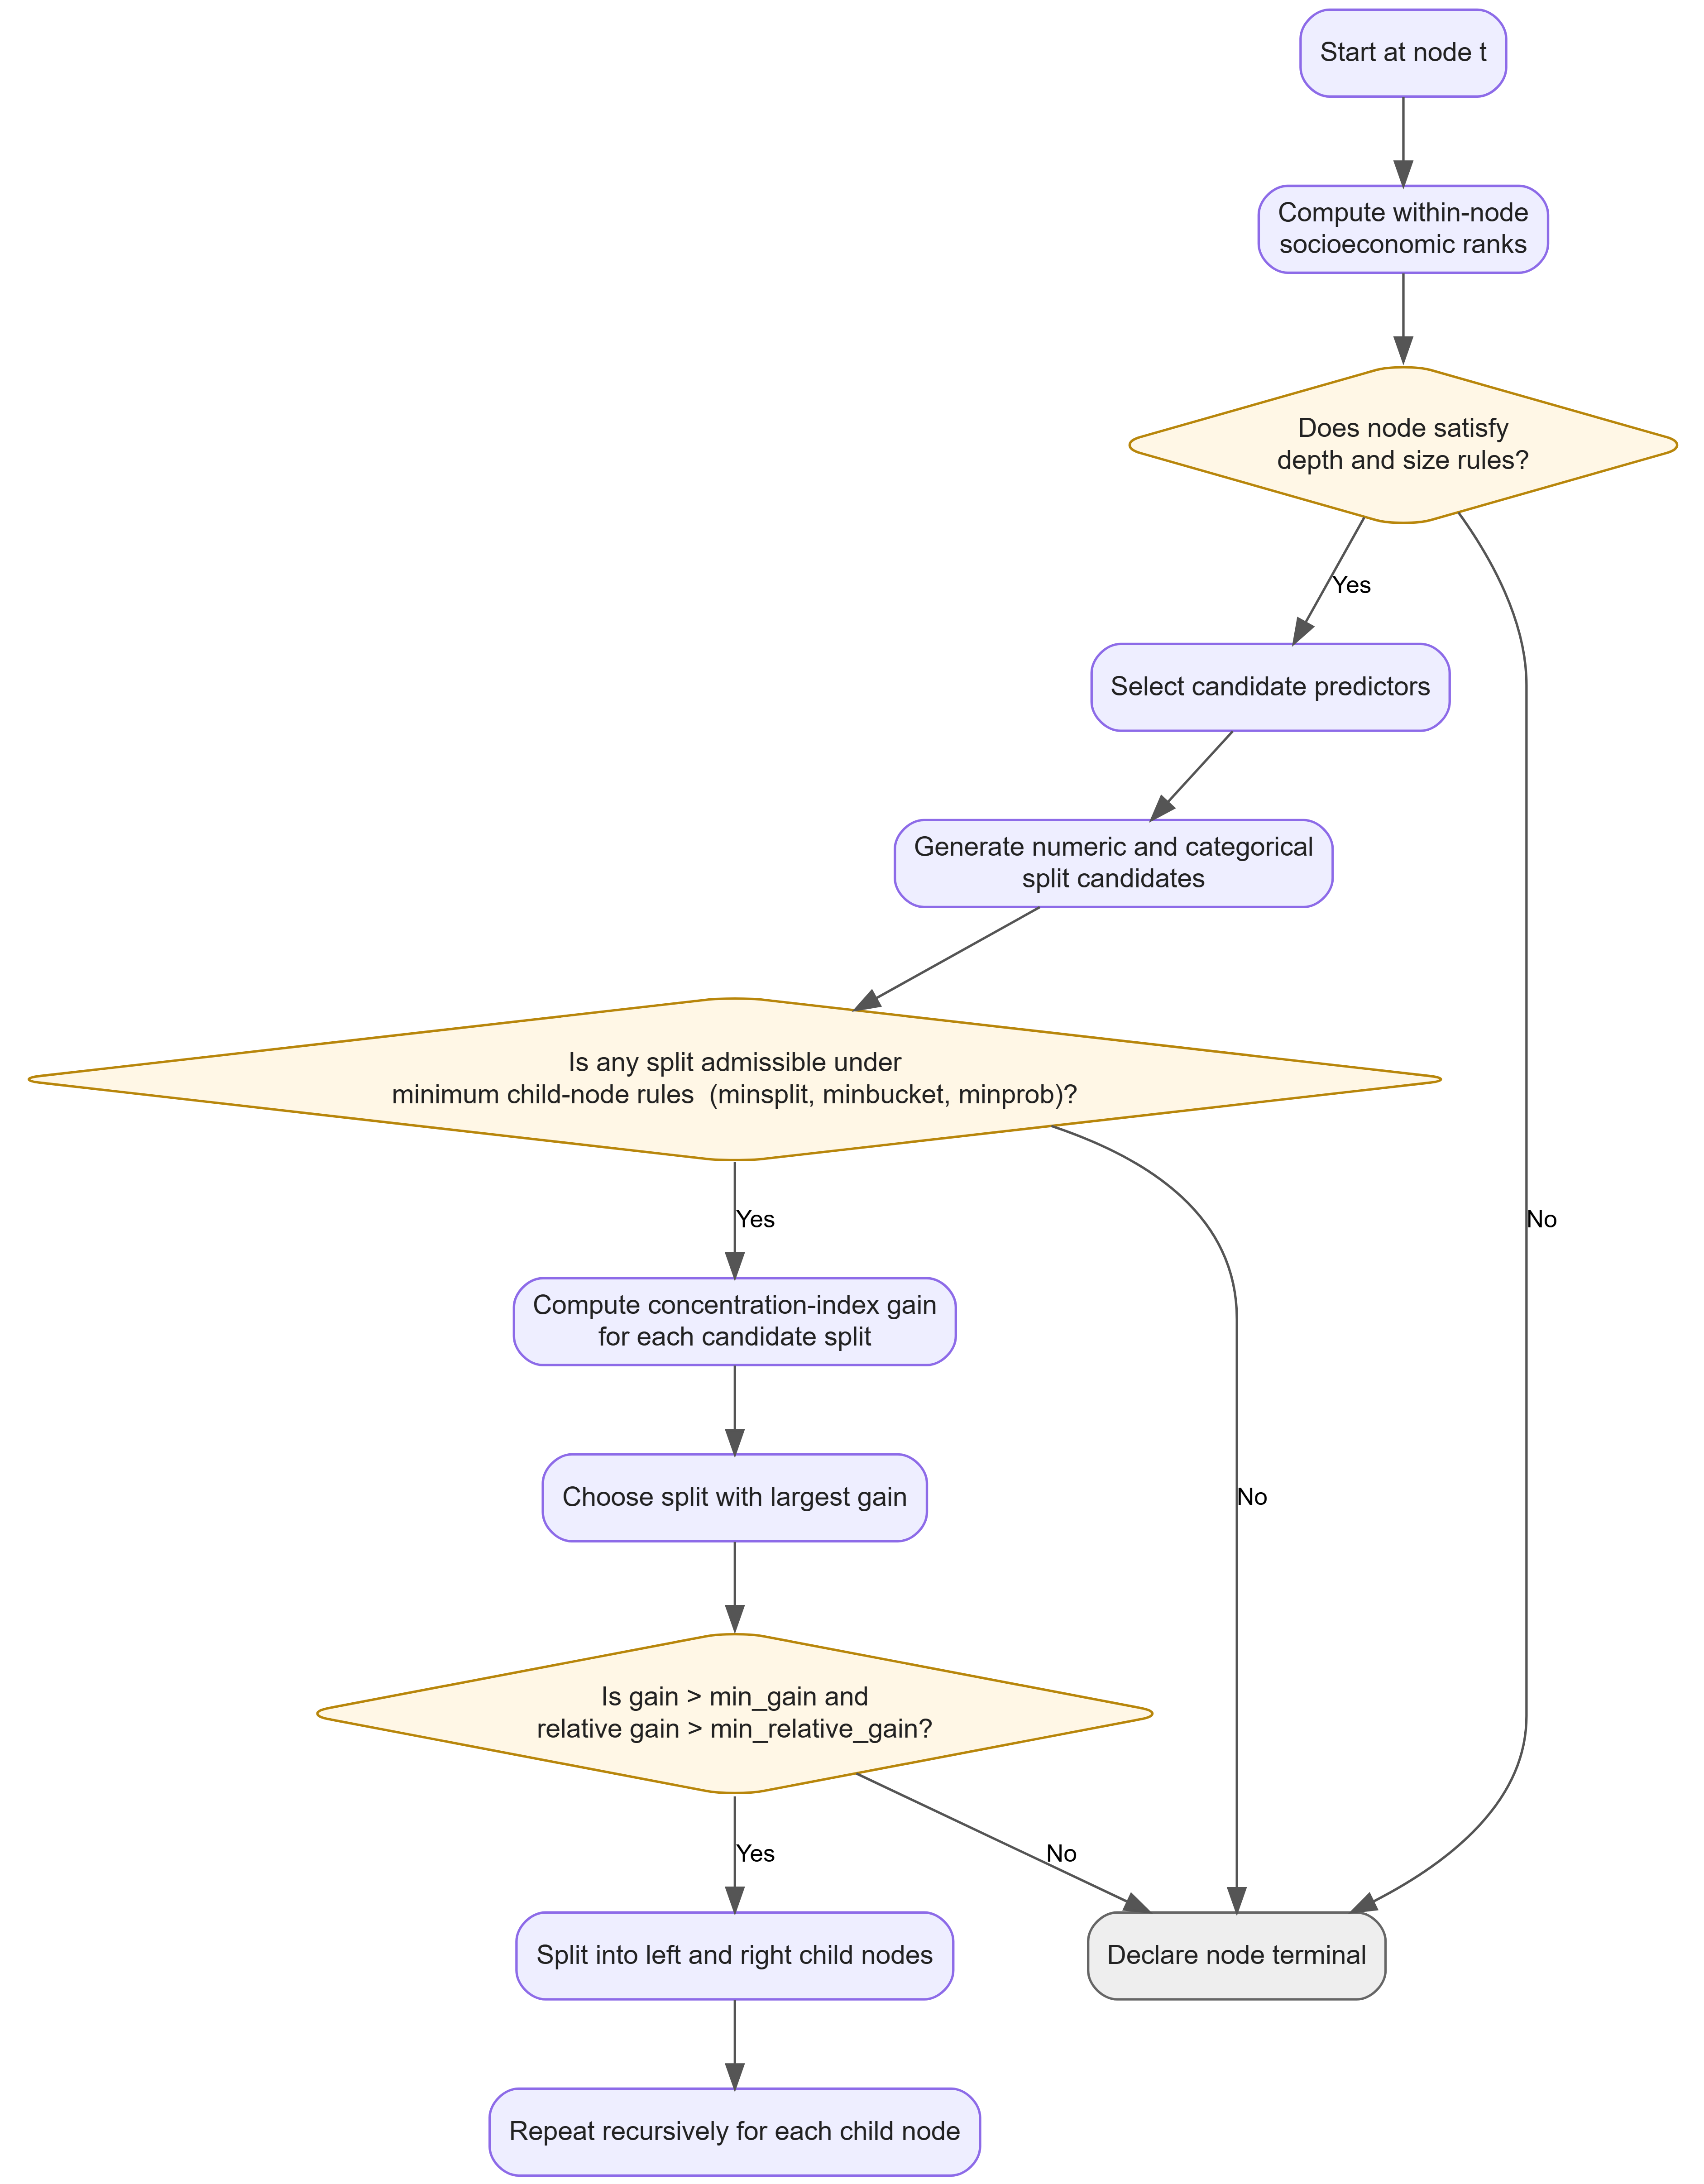
\includegraphics[width=5.5in,height=7in]{MSE_Thesis_Decomposition_of_CI_Trees_MM_files/figure-latex/dot-figure-1.png}

}

\caption{\label{fig-greedy-ci-tree-flow}Greedy concentration-index
tree-growing procedure.}

\end{figure}%

\subsection{Results}\label{results-1}

\subsubsection{Appendix R1: Exploratory Data
Outputs}\label{appendix-r1-exploratory-data-outputs}

\begingroup\fontsize{11}{13}\selectfont

\begin{longtable}[t]{>{\raggedright\arraybackslash}p{4.5cm}>{\raggedleft\arraybackslash}p{3.1cm}>{\raggedleft\arraybackslash}p{3.1cm}>{\raggedleft\arraybackslash}p{3.1cm}}

\caption{\label{tbl-appendix-weighted-baseline}Weighted distribution of
analysis variables by under-five mortality status}

\tabularnewline

\\
\toprule
\multicolumn{1}{c}{\textbf{ }} & \multicolumn{2}{c}{\textbf{Under-five mortality}} & \multicolumn{1}{c}{\textbf{Overall}} \\
\cmidrule(l{3pt}r{3pt}){2-3} \cmidrule(l{3pt}r{3pt}){4-4}
\textbf{Variable} & \textbf{Alive at age 5} & \textbf{Died before age 5} & \textbf{Overall}\\
\midrule
 & (weighted N=7,464) & (weighted N=859) & (weighted N=8,323)\\
Household wealth &  &  & \\
High household wealth & 4,266.9 (57.2\%) & 418.6 (48.7\%) & 4,685.5 (56.3\%)\\
Low household wealth & 3,197.4 (42.8\%) & 440.2 (51.3\%) & 3,637.6 (43.7\%)\\
Skilled.birth.attendance &  &  & \\
\addlinespace
Skilled.birth.attendance.1 & 3,225.3 (43.2\%) & 295.1 (34.4\%) & 3,520.5 (42.3\%)\\
No.skilled.birth.attendance & 4,239 (56.8\%) & 563.6 (65.6\%) & 4,802.6 (57.7\%)\\
Sex of the child &  &  & \\
Female & 3,828.8 (51.3\%) & 390.4 (45.5\%) & 4,219.2 (50.7\%)\\
Male & 3,635.5 (48.7\%) & 468.4 (54.5\%) & 4,103.9 (49.3\%)\\
\addlinespace
Birth order and interval &  &  & \\
First birth & 1,396.8 (18.7\%) & 190.9 (22.2\%) & 1,587.7 (19.1\%)\\
2-4 short interval & 774.3 (10.4\%) & 110.1 (12.8\%) & 884.4 (10.6\%)\\
2-4 long interval & 2,603.8 (34.9\%) & 216.6 (25.2\%) & 2,820.3 (33.9\%)\\
5+ short interval & 696.6 (9.3\%) & 150.6 (17.5\%) & 847.2 (10.2\%)\\
\addlinespace
5+ long interval & 1,992.8 (26.7\%) & 190.7 (22.2\%) & 2,183.5 (26.2\%)\\
Mother's age at birth &  &  & \\
20 or more & 4,256.1 (57.0\%) & 472.6 (55.0\%) & 4,728.8 (56.8\%)\\
Less than 20 & 3,208.1 (43.0\%) & 386.2 (45.0\%) & 3,594.3 (43.2\%)\\
Type of residence &  &  & \\
\addlinespace
Urban & 2,932.1 (39.3\%) & 263.6 (30.7\%) & 3,195.7 (38.4\%)\\
Rural & 4,532.2 (60.7\%) & 595.2 (69.3\%) & 5,127.4 (61.6\%)\\
Mother's education &  &  & \\
Any education & 3,342.9 (44.8\%) & 278.8 (32.5\%) & 3,621.8 (43.5\%)\\
No education & 4,121.4 (55.2\%) & 579.9 (67.5\%) & 4,701.3 (56.5\%)\\
\addlinespace
Father's education &  &  & \\
Any education & 5,490 (73.6\%) & 589.1 (68.6\%) & 6,079.2 (73.0\%)\\
No education & 1,974.3 (26.4\%) & 269.7 (31.4\%) & 2,243.9 (27.0\%)\\
Mother's occupation &  &  & \\
Other & 1,610.2 (21.6\%) & 135.1 (15.7\%) & 1,745.4 (21.0\%)\\
\addlinespace
Household, unskilled, not working & 1,757.2 (23.5\%) & 172.1 (20.0\%) & 1,929.4 (23.2\%)\\
Agriculture & 4,096.8 (54.9\%) & 551.6 (64.2\%) & 4,648.4 (55.8\%)\\
Father's occupation &  &  & \\
Other & 2,810.3 (37.6\%) & 242.1 (28.2\%) & 3,052.4 (36.7\%)\\
Household, unskilled, not working & 961.3 (12.9\%) & 108.5 (12.6\%) & 1,069.8 (12.9\%)\\
\addlinespace
Agriculture & 3,692.7 (49.5\%) & 508.1 (59.2\%) & 4,200.9 (50.5\%)\\
\bottomrule

\end{longtable}

\endgroup{}

\begin{figure}[H]

\centering{

\pandocbounded{
\includegraphics[keepaspectratio]{MSE_Thesis_Decomposition_of_CI_Trees_MM_files/figure-pdf/fig-appendix-province-mortality-distribution-1.pdf}}

}

\caption{\label{fig-appendix-province-mortality-distribution}Weighted
province distribution by under-five mortality status.}

\end{figure}%

\subsubsection{Appendix R2: Regression and Predictive-Forest
Details}\label{appendix-r2-regression-and-predictive-forest-details}

\paragraph{Regression model summary}\label{regression-model-summary}

\begingroup\fontsize{11}{13}\selectfont

\begin{longtable}[t]{>{\raggedright\arraybackslash}p{4.5cm}rrrlrr}

\caption{\label{tbl-appendix-regression-model-summary}Survey-weighted
regression model summary}

\tabularnewline

\\
\toprule
\textbf{Term} & \textbf{Estimate} & \textbf{Std. error} & \textbf{Statistic} & \textbf{p-value} & \textbf{Conf. low} & \textbf{Conf. high}\\
\midrule
Intercept & -2.908 & 0.282 & -10.319 & < 0.001 & -3.463 & -2.354\\
Household wealth & 0.068 & 0.118 & 0.579 & 0.56311 & -0.164 & 0.300\\
Skilled birth attendance & 0.198 & 0.134 & 1.479 & 0.14018 & -0.066 & 0.462\\
Sex of the child & 0.242 & 0.084 & 2.864 & 0.00451 & 0.076 & 0.408\\
Birth order and interval: 2-4 short interval & -0.004 & 0.165 & -0.023 & 0.98177 & -0.328 & 0.320\\
\addlinespace
Birth order and interval: 2-4 long interval & -0.509 & 0.136 & -3.742 & < 0.001 & -0.777 & -0.241\\
Birth order and interval: 5+ short interval & 0.420 & 0.187 & 2.247 & 0.02543 & 0.052 & 0.787\\
Birth order and interval: 5+ long interval & -0.396 & 0.189 & -2.096 & 0.03701 & -0.769 & -0.024\\
Mother's age at birth & 0.033 & 0.152 & 0.215 & 0.82980 & -0.267 & 0.332\\
Type of residence & 0.090 & 0.135 & 0.667 & 0.50556 & -0.176 & 0.356\\
\addlinespace
Mother's education & 0.336 & 0.120 & 2.799 & 0.00549 & 0.100 & 0.573\\
Father's education & -0.036 & 0.119 & -0.300 & 0.76476 & -0.270 & 0.199\\
Mother's occupation: Household, unskilled, not working & -0.018 & 0.159 & -0.112 & 0.91123 & -0.330 & 0.294\\
Mother's occupation: Agriculture & 0.140 & 0.181 & 0.776 & 0.43864 & -0.216 & 0.497\\
Father's occupation: Household, unskilled, not working & 0.235 & 0.144 & 1.638 & 0.10253 & -0.048 & 0.518\\
\addlinespace
Father's occupation: Agriculture & 0.225 & 0.143 & 1.577 & 0.11587 & -0.056 & 0.506\\
Region: Bas-Congo & 0.258 & 0.260 & 0.993 & 0.32139 & -0.253 & 0.769\\
Region: Equateur & 0.250 & 0.283 & 0.882 & 0.37862 & -0.308 & 0.807\\
Region: Kasai Occidental & 0.105 & 0.269 & 0.391 & 0.69603 & -0.424 & 0.634\\
Region: Kasai Oriental & 0.153 & 0.212 & 0.719 & 0.47266 & -0.265 & 0.571\\
\addlinespace
Region: Katanga & 0.515 & 0.256 & 2.014 & 0.04499 & 0.012 & 1.018\\
Region: Kinshasa & 0.081 & 0.288 & 0.283 & 0.77733 & -0.485 & 0.648\\
Region: Maniema & 0.489 & 0.235 & 2.084 & 0.03808 & 0.027 & 0.951\\
Region: Nord-Kivu & -0.252 & 0.319 & -0.789 & 0.43053 & -0.879 & 0.376\\
Region: Orientale & -0.084 & 0.295 & -0.283 & 0.77728 & -0.665 & 0.498\\
\addlinespace
Region: Sud-Kivu & 0.300 & 0.251 & 1.194 & 0.23338 & -0.194 & 0.794\\
\bottomrule

\end{longtable}

\endgroup{}

\paragraph{Predictive ranger tuning
results}\label{predictive-ranger-tuning-results}

\begingroup\fontsize{11}{13}\selectfont

\begin{longtable}[t]{llrrr}

\caption{\label{tbl-appendix-ranger-sampling-summary}Weighted class
distribution before and after ranger undersampling}

\tabularnewline

\\
\toprule
\textbf{Sample} & \textbf{Outcome} & \textbf{Rows} & \textbf{Weighted N} & \textbf{Weighted percent}\\
\midrule
Before undersampling & Alive at age 5 & 7424 & 7464.30 & 89.68\\
Before undersampling & Died before age 5 & 872 & 858.80 & 10.32\\
After undersampling & Alive at age 5 & 1274 & 1289.74 & 60.03\\
After undersampling & Died before age 5 & 872 & 858.80 & 39.97\\
\bottomrule

\end{longtable}

\endgroup{}

\begingroup\fontsize{11}{13}\selectfont

\begin{longtable}[t]{>{\raggedright\arraybackslash}p{2.4cm}rrrrrr}

\caption{\label{tbl-appendix-ranger-cross-validation}Cross-validation
results for the predictive ranger model}

\tabularnewline

\\
\toprule
\textbf{Metric} & \textbf{mtry} & \textbf{min\_n} & \textbf{Mean} & \textbf{Std. error} & \textbf{Folds} & \textbf{Rank}\\
\midrule
accuracy & 10 & 800 & 0.5896 & 0.0221 & 10 & 1\\
accuracy & 22 & 200 & 0.5849 & 0.0166 & 10 & 2\\
accuracy & 29 & 500 & 0.5844 & 0.0191 & 10 & 3\\
accuracy & 16 & 800 & 0.5836 & 0.0203 & 10 & 4\\
accuracy & 10 & 500 & 0.5820 & 0.0223 & 10 & 5\\
\addlinespace
accuracy & 22 & 800 & 0.5808 & 0.0161 & 10 & 6\\
accuracy & 16 & 200 & 0.5806 & 0.0170 & 10 & 7\\
accuracy & 22 & 500 & 0.5782 & 0.0209 & 10 & 8\\
accuracy & 10 & 200 & 0.5781 & 0.0184 & 10 & 9\\
accuracy & 29 & 200 & 0.5767 & 0.0153 & 10 & 10\\
\addlinespace
accuracy & 16 & 500 & 0.5765 & 0.0214 & 10 & 11\\
accuracy & 29 & 800 & 0.5757 & 0.0158 & 10 & 12\\
f\_meas & 22 & 200 & 0.3776 & 0.0214 & 10 & 1\\
f\_meas & 29 & 200 & 0.3730 & 0.0209 & 10 & 2\\
f\_meas & 16 & 200 & 0.3627 & 0.0216 & 10 & 3\\
\addlinespace
f\_meas & 10 & 200 & 0.3380 & 0.0207 & 10 & 4\\
f\_meas & 29 & 500 & 0.3358 & 0.0258 & 10 & 5\\
f\_meas & 22 & 500 & 0.3195 & 0.0300 & 10 & 6\\
f\_meas & 16 & 500 & 0.2945 & 0.0296 & 10 & 7\\
f\_meas & 10 & 500 & 0.2769 & 0.0305 & 10 & 8\\
\addlinespace
f\_meas & 29 & 800 & 0.2498 & 0.0393 & 10 & 9\\
f\_meas & 22 & 800 & 0.2442 & 0.0374 & 10 & 10\\
f\_meas & 16 & 800 & 0.2315 & 0.0360 & 10 & 11\\
f\_meas & 10 & 800 & 0.1924 & 0.0348 & 10 & 12\\
roc\_auc & 10 & 500 & 0.6012 & 0.0114 & 10 & 1\\
\addlinespace
roc\_auc & 16 & 800 & 0.6002 & 0.0111 & 10 & 2\\
roc\_auc & 16 & 200 & 0.5997 & 0.0093 & 10 & 3\\
roc\_auc & 16 & 500 & 0.5995 & 0.0101 & 10 & 4\\
roc\_auc & 29 & 800 & 0.5994 & 0.0094 & 10 & 5\\
roc\_auc & 10 & 800 & 0.5993 & 0.0120 & 10 & 6\\
\addlinespace
roc\_auc & 22 & 500 & 0.5991 & 0.0094 & 10 & 7\\
roc\_auc & 22 & 200 & 0.5986 & 0.0099 & 10 & 8\\
roc\_auc & 22 & 800 & 0.5983 & 0.0104 & 10 & 9\\
roc\_auc & 29 & 200 & 0.5980 & 0.0092 & 10 & 10\\
roc\_auc & 10 & 200 & 0.5980 & 0.0103 & 10 & 11\\
\addlinespace
roc\_auc & 29 & 500 & 0.5977 & 0.0088 & 10 & 12\\
sensitivity & 22 & 200 & 0.3074 & 0.0296 & 10 & 1\\
sensitivity & 29 & 200 & 0.3074 & 0.0287 & 10 & 2\\
sensitivity & 16 & 200 & 0.2913 & 0.0284 & 10 & 3\\
sensitivity & 10 & 200 & 0.2627 & 0.0269 & 10 & 4\\
\addlinespace
sensitivity & 29 & 500 & 0.2593 & 0.0322 & 10 & 5\\
sensitivity & 22 & 500 & 0.2467 & 0.0345 & 10 & 6\\
sensitivity & 16 & 500 & 0.2204 & 0.0330 & 10 & 7\\
sensitivity & 29 & 800 & 0.1987 & 0.0543 & 10 & 8\\
sensitivity & 10 & 500 & 0.1986 & 0.0307 & 10 & 9\\
\addlinespace
sensitivity & 22 & 800 & 0.1860 & 0.0477 & 10 & 10\\
sensitivity & 16 & 800 & 0.1653 & 0.0384 & 10 & 11\\
sensitivity & 10 & 800 & 0.1240 & 0.0280 & 10 & 12\\
spec & 10 & 800 & 0.9457 & 0.0152 & 10 & 1\\
spec & 16 & 800 & 0.9127 & 0.0227 & 10 & 2\\
\addlinespace
spec & 22 & 800 & 0.8967 & 0.0323 & 10 & 3\\
spec & 29 & 800 & 0.8826 & 0.0364 & 10 & 4\\
spec & 10 & 500 & 0.8783 & 0.0178 & 10 & 5\\
spec & 16 & 500 & 0.8539 & 0.0218 & 10 & 6\\
spec & 22 & 500 & 0.8367 & 0.0230 & 10 & 7\\
\addlinespace
spec & 29 & 500 & 0.8365 & 0.0224 & 10 & 8\\
spec & 10 & 200 & 0.8227 & 0.0208 & 10 & 9\\
spec & 16 & 200 & 0.8045 & 0.0217 & 10 & 10\\
spec & 22 & 200 & 0.8005 & 0.0229 & 10 & 11\\
spec & 29 & 200 & 0.7859 & 0.0216 & 10 & 12\\
\bottomrule

\end{longtable}

\endgroup{}

\paragraph{Predictive ranger SHAP summary
plot}\label{predictive-ranger-shap-summary-plot}

\begin{figure}[H]

\centering{

\pandocbounded{
\includegraphics[keepaspectratio]{MSE_Thesis_Decomposition_of_CI_Trees_MM_files/figure-pdf/fig-appendix-shap-summary-1.pdf}}

}

\caption{\label{fig-appendix-shap-summary}SHAP summary plot for the
predictive ranger model.}

\end{figure}%

\subsubsection{Appendix R3: Concentration-Index Tree
Details}\label{appendix-r3-concentration-index-tree-details}

\paragraph{Tree tuning and selection
details}\label{tree-tuning-and-selection-details}

\begingroup\fontsize{11}{13}\selectfont

\begin{longtable}[t]{lrrrrrr}

\caption{\label{tbl-appendix-tree-best-controls}Best tree
hyperparameters selected by validation gain within each impurity
criterion}

\tabularnewline

\\
\toprule
\textbf{type} & \textbf{minsplit} & \textbf{minbucket} & \textbf{minprob} & \textbf{maxdepth} & \textbf{min\_gain} & \textbf{min\_relative\_gain}\\
\midrule
CI & 500 & 100 & 0.01 & 10 & 1e-04 & 0.25\\
CIg & 500 & 100 & 0.01 & 10 & 1e-04 & 0.30\\
CIc & 500 & 100 & 0.01 & 10 & 1e-04 & 0.30\\
L & 500 & 100 & 0.01 & 10 & 1e-04 & 0.25\\
\bottomrule

\end{longtable}

\endgroup{}

\paragraph{Tree fit and selection
summaries}\label{tree-fit-and-selection-summaries}

\begingroup\fontsize{11}{13}\selectfont

\begin{longtable}[t]{llrr}

\caption{\label{tbl-appendix-tree-selected-setting-summary}Tree summary
for the selected settings}

\tabularnewline

\\
\toprule
\textbf{criterion} & \textbf{metric} & \textbf{estimate} & \textbf{std\_error}\\
\midrule
CI & Root impurity & 0.1293 & NA\\
CI & Training gain & 0.0960 & 0.0044\\
CI & Training gain (\% root) & 83.3135 & 1.6199\\
CI & Validation gain & -0.0234 & 0.0189\\
CI & Validation gain (\% root) & -1157.1539 & 1131.8743\\
\addlinespace
CIc & Root impurity & 0.0591 & NA\\
CIc & Training gain & 0.0388 & 0.0019\\
CIc & Training gain (\% root) & 81.5691 & 2.1079\\
CIc & Validation gain & -0.0030 & 0.0077\\
CIc & Validation gain (\% root) & -1058.0175 & 1039.5234\\
\addlinespace
CIg & Root impurity & 0.0148 & NA\\
CIg & Training gain & 0.0097 & 0.0005\\
CIg & Training gain (\% root) & 81.5691 & 2.1079\\
CIg & Validation gain & -0.0007 & 0.0019\\
CIg & Validation gain (\% root) & -1058.0175 & 1039.5234\\
\addlinespace
L & Root impurity & 1.8028 & NA\\
L & Training gain & 0.1995 & 0.0174\\
L & Training gain (\% root) & 98.1872 & 0.3555\\
L & Validation gain & 1.7776 & 1.6048\\
L & Validation gain (\% root) & 64.4907 & 11.3190\\
\bottomrule

\end{longtable}

\endgroup{}

\paragraph{Tree selection metrics}\label{tree-selection-metrics}

\begingroup\fontsize{11}{13}\selectfont

\begin{longtable}[t]{>{\raggedright\arraybackslash}p{1.4cm}>{\raggedleft\arraybackslash}p{1.8cm}>{\raggedleft\arraybackslash}p{1.8cm}>{\raggedleft\arraybackslash}p{1.8cm}>{\raggedleft\arraybackslash}p{1.8cm}>{\raggedleft\arraybackslash}p{1.8cm}>{\raggedleft\arraybackslash}p{1.8cm}}

\caption{\label{tbl-appendix-tree-selection}Selection metrics for fitted
concentration-index trees}

\tabularnewline

\\
\toprule
\textbf{Criterion} & \textbf{Root objective} & \textbf{Train gain} & \textbf{Train gain/root} & \textbf{Validation gain} & \textbf{Validation gain/root} & \textbf{Terminal nodes}\\
\midrule
CI & 0.1293 & 0.0960 & 0.8331 & -0.0234 & -11.5715 & 6.9\\
CIc & 0.0591 & 0.0388 & 0.8157 & -0.0030 & -10.5802 & 6.0\\
CIg & 0.0148 & 0.0097 & 0.8157 & -0.0007 & -10.5802 & 6.0\\
L & 1.8028 & 0.1995 & 0.9819 & 1.7776 & 0.6449 & 7.5\\
\bottomrule

\end{longtable}

\endgroup{}

\begin{figure}[H]

\centering{

\pandocbounded{
\includegraphics[keepaspectratio]{MSE_Thesis_Decomposition_of_CI_Trees_MM_files/figure-pdf/fig-appendix-tree-variable-importance-1.pdf}}

}

\caption{\label{fig-appendix-tree-variable-importance}Top tree variables
by concentration-index criterion.}

\end{figure}%

\subsubsection{Additional Concentration-Index Tree
Plots}\label{additional-concentration-index-tree-plots}

\begin{figure}[H]

\centering{

\pandocbounded{
\includegraphics[keepaspectratio]{MSE_Thesis_Decomposition_of_CI_Trees_MM_files/figure-pdf/fig-appendix-ci-tree-cig-1.pdf}}

}

\caption{\label{fig-appendix-ci-tree-cig}Concentration-index tree fitted
with the CIg criterion.}

\end{figure}%

\begin{figure}[H]

\centering{

\pandocbounded{
\includegraphics[keepaspectratio]{MSE_Thesis_Decomposition_of_CI_Trees_MM_files/figure-pdf/fig-appendix-ci-tree-ci-1.pdf}}

}

\caption{\label{fig-appendix-ci-tree-ci}Concentration-index tree fitted
with the CI criterion.}

\end{figure}%

\subsubsection{Appendix R4: Rpart Comparison Tree
Details}\label{appendix-r4-rpart-comparison-tree-details}

\begin{figure}[H]

\centering{

\pandocbounded{
\includegraphics[keepaspectratio]{MSE_Thesis_Decomposition_of_CI_Trees_MM_files/figure-pdf/fig-appendix-lecturer-rpart-simple-1.pdf}}

}

\caption{\label{fig-appendix-lecturer-rpart-simple}Rpart comparison tree
using absolute CI impurity.}

\end{figure}%

\subsubsection{Appendix 5: Concentration-Index Forest
Details}\label{appendix-5-concentration-index-forest-details}

\paragraph{Forest tuning and selection
details}\label{forest-tuning-and-selection-details}

\begingroup\fontsize{11}{13}\selectfont

\begin{longtable}[t]{lrrrrrrrr}

\caption{\label{tbl-appendix-forest-best-controls}Best forest
hyperparameters selected by validation gain within each impurity
criterion}

\tabularnewline

\\
\toprule
\textbf{type} & \textbf{ntree} & \textbf{mtry} & \textbf{minsplit} & \textbf{minbucket} & \textbf{minprob} & \textbf{maxdepth} & \textbf{min gain} & \textbf{min relative gain}\\
\midrule
CI & 100 & 15 & 500 & 100 & 0.01 & 15 & 0 & 0.25\\
CIc & 100 & 15 & 500 & 100 & 0.01 & 15 & 0 & 0.25\\
CIg & 100 & 15 & 500 & 100 & 0.01 & 15 & 0 & 0.25\\
L & 50 & 15 & 500 & 100 & 0.01 & 15 & 0 & 0.20\\
\bottomrule

\end{longtable}

\endgroup{}

\paragraph{Forest fit and selection
summaries}\label{forest-fit-and-selection-summaries}

\begingroup\fontsize{11}{13}\selectfont

\begin{longtable}[t]{llrr}

\caption{\label{tbl-appendix-forest-selected-setting-summary}Forest
summary for the selected settings}

\tabularnewline

\\
\toprule
\textbf{criterion} & \textbf{metric} & \textbf{estimate} & \textbf{std\_error}\\
\midrule
CI & Root impurity & 0.1293 & NA\\
CI & Training gain & 0.0553 & 0.0031\\
CI & Training gain (\% root) & 48.1137 & 1.9835\\
CI & Validation gain & -0.0137 & 0.0147\\
CI & Validation gain (\% root) & -1038.2520 & 1024.0575\\
\addlinespace
CIc & Root impurity & 0.0591 & NA\\
CIc & Training gain & 0.0245 & 0.0011\\
CIc & Training gain (\% root) & 51.7127 & 1.8192\\
CIc & Validation gain & -0.0012 & 0.0075\\
CIc & Validation gain (\% root) & -1108.4715 & 1101.3651\\
\addlinespace
CIg & Root impurity & 0.0148 & NA\\
CIg & Training gain & 0.0061 & 0.0003\\
CIg & Training gain (\% root) & 51.5535 & 1.9667\\
CIg & Validation gain & -0.0001 & 0.0019\\
CIg & Validation gain (\% root) & -1063.0446 & 1055.1327\\
\addlinespace
L & Root impurity & 1.8028 & NA\\
L & Training gain & 0.1941 & 0.0173\\
L & Training gain (\% root) & 95.2953 & 0.6298\\
L & Validation gain & 1.7544 & 1.5950\\
L & Validation gain (\% root) & 56.6798 & 11.5910\\
\bottomrule

\end{longtable}

\endgroup{}

\paragraph{Forest selection metrics}\label{forest-selection-metrics}

\begingroup\fontsize{11}{13}\selectfont

\begin{longtable}[t]{>{\raggedright\arraybackslash}p{1.4cm}>{\raggedleft\arraybackslash}p{1.8cm}>{\raggedleft\arraybackslash}p{1.8cm}>{\raggedleft\arraybackslash}p{1.8cm}>{\raggedleft\arraybackslash}p{1.8cm}>{\raggedleft\arraybackslash}p{1.8cm}>{\raggedleft\arraybackslash}p{1.8cm}}

\caption{\label{tbl-appendix-forest-selection}Selection metrics for
fitted concentration-index forests}

\tabularnewline

\\
\toprule
\textbf{Criterion} & \textbf{Root objective} & \textbf{Train gain} & \textbf{Train gain/root} & \textbf{Validation gain} & \textbf{Validation gain/root} & \textbf{Mean terminal nodes}\\
\midrule
CI & 0.1293 & 0.0553 & 0.4811 & -0.0137 & -10.3825 & 4.014\\
CIc & 0.0591 & 0.0245 & 0.5171 & -0.0012 & -11.0847 & 4.113\\
CIg & 0.0148 & 0.0061 & 0.5155 & -0.0001 & -10.6304 & 4.148\\
L & 1.8028 & 0.1941 & 0.9530 & 1.7544 & 0.5668 & 5.448\\
\bottomrule

\end{longtable}

\endgroup{}

\paragraph{Forest complexity plots}\label{forest-complexity-plots}

\begin{figure}[H]

\centering{

\pandocbounded{
\includegraphics[keepaspectratio]{MSE_Thesis_Decomposition_of_CI_Trees_MM_files/figure-pdf/fig-appendix-forest-complexity-path-1.pdf}}

}

\caption{\label{fig-appendix-forest-complexity-path}Forest complexity by
number of terminal nodes.}

\end{figure}%

\begin{figure}[H]

\centering{

\pandocbounded{
\includegraphics[keepaspectratio]{MSE_Thesis_Decomposition_of_CI_Trees_MM_files/figure-pdf/fig-appendix-forest-variable-importance-1.pdf}}

}

\caption{\label{fig-appendix-forest-variable-importance}Top forest
variables by concentration-index criterion.}

\end{figure}%

\paragraph{Forest Surrogate Trees
plots}\label{forest-surrogate-trees-plots}

The selected forest surrogate appears in the results section. The
remaining criterion-specific forest surrogates are retained here for
comparison.

\begin{figure}[H]

\centering{

\pandocbounded{
\includegraphics[keepaspectratio]{MSE_Thesis_Decomposition_of_CI_Trees_MM_files/figure-pdf/fig-appendix-forest-surrogate-ci-1.pdf}}

}

\caption{\label{fig-appendix-forest-surrogate-ci}Surrogate tree for the
CI concentration-index forest.}

\end{figure}%

\begin{figure}[H]

\centering{

\pandocbounded{
\includegraphics[keepaspectratio]{MSE_Thesis_Decomposition_of_CI_Trees_MM_files/figure-pdf/fig-appendix-forest-surrogate-cig-1.pdf}}

}

\caption{\label{fig-appendix-forest-surrogate-cig}Surrogate tree for the
CIg concentration-index forest.}

\end{figure}%

\begin{figure}[H]

\centering{

\pandocbounded{
\includegraphics[keepaspectratio]{MSE_Thesis_Decomposition_of_CI_Trees_MM_files/figure-pdf/fig-appendix-forest-surrogate-cic-1.pdf}}

}

\caption{\label{fig-appendix-forest-surrogate-cic}Surrogate tree for the
CIc concentration-index forest.}

\end{figure}%

\begin{figure}[H]

\centering{

\pandocbounded{
\includegraphics[keepaspectratio]{MSE_Thesis_Decomposition_of_CI_Trees_MM_files/figure-pdf/fig-appendix-forest-surrogate-l-1.pdf}}

}

\caption{\label{fig-appendix-forest-surrogate-l}Surrogate tree for the L
concentration-index forest.}

\end{figure}%

\subsubsection{Appendix S: Simulation Sensitivity
Plots}\label{appendix-s-simulation-sensitivity-plots}

The CIg tree is shown in the main results section. The remaining
positive-control simulation trees are shown here to check whether the
recovered subgroup pattern is stable across concentration-index
criteria.

\begin{figure}[H]

\centering{

\pandocbounded{
\includegraphics[keepaspectratio]{MSE_Thesis_Decomposition_of_CI_Trees_MM_files/figure-pdf/fig-appendix-simulation-positive-control-ci-1.pdf}}

}

\caption{\label{fig-appendix-simulation-positive-control-ci}Positive-control
simulation tree fitted with the CI criterion.}

\end{figure}%

\begin{figure}[H]

\centering{

\pandocbounded{
\includegraphics[keepaspectratio]{MSE_Thesis_Decomposition_of_CI_Trees_MM_files/figure-pdf/fig-appendix-simulation-positive-control-cic-1.pdf}}

}

\caption{\label{fig-appendix-simulation-positive-control-cic}Positive-control
simulation tree fitted with the CIc criterion.}

\end{figure}%

\begin{figure}[H]

\centering{

\pandocbounded{
\includegraphics[keepaspectratio]{MSE_Thesis_Decomposition_of_CI_Trees_MM_files/figure-pdf/fig-appendix-simulation-positive-control-l-1.pdf}}

}

\caption{\label{fig-appendix-simulation-positive-control-l}Positive-control
simulation tree fitted with the L criterion.}

\end{figure}%




\end{document}
